\documentclass[../full_thesis/full_thesis.tex]{subfiles}

% Default image directory
\newcommand{\thisdir}{../analytic_timing_noise_cgw}
\graphicspath{{\thisdir/img/}}

\begin{document}

It's unclear at this time what causes timing noise, but from
Chapter~\ref{sec: timing noise in cgw} we know that it may pose a problem for
continuous GW searches if the phase evolution is effected by timing noise and
this is not included in the search templates. In addition to searches for
isolated neutron stars, many searches \citep[see for
example][]{ligo2015scox1,leaci2015,ScoX1:MDC1} have been performed for GWs from
low-mass X-ray binary systems (LMXBs). These searches experience similar
difficulties due to a stronger form of timing noise known as `spin-wandering'.
This issue was investigated by \citet{watts2008} who quantified the effect for
a spin-up of $\dot{\nu}_{\textrm{s}}$ by defining a decoherence time
$T_{\textrm{decoh}}^{2} \dot{\nu}_{\textrm{s}} = 1$, after which the Taylor
expansion can no longer track the phase.  They then estimated a worst-case
decoherence time by using the maximal spin-up rate due to the accretion torque
and found that for some sources such as the LMXB Scorpius-X1, the decoherence
time can be short as $\sim 1$~week.

In this chapter, we will present some preliminary calculations and results
related to modelling timing noise in a continuous GW using a random walk model.
Unlike the results of Chapter~\ref{sec: timing noise in cgw}, which used an
empirical description of timing noise given by the Crab ephemeris, the results
derived here can be applied to any search in which it is thought the signal may
undergo a random walk. In this sense, it is equivalent to Chapter~\ref{sec:
glitches in cgw} in that the ultimate aim is to estimate the risk faced by
various searches by inferring from the observed pulsar population.  As given
here, the task in incomplete and so we will present our calculations and
some preliminary results.

Recent observations by \citet{Hobbs2010} suggest that a random walk model does
not capture the physics of timing noise in isolated radio pulsars and hence is
not a useful way to infer neutron star physics. Nevertheless, the random walk
model remains a practical empirical model; in this section then, we use it as
such without requiring it to have any deeper substantive meaning for what
causes timing noise. In the same way, the random walk model can also be applied
to LMXBs where the amount of spin-wandering could be inferred from fluctuations
in the luminosity. From this, we would like in the future to update the estimates by
\citet{watts2008} to estimate the mismatch for searches for continuous gravitational
waves from LMXBs.

This chapter is organised in the following way. In Section~\ref{sec: defining a
random walk} we will define the random walk as a piecewise Taylor expansion in
which the difference between the signal and template is initially zero. We will
then calculate the mismatch for this simple description in Section~\ref{sec:
random walk models part I}. However, setting the difference between the signal
and template to zero initially does not minimise the mismatch, so in
Section~\ref{sec: random walk models part II} we will discuss a pragmatic
method to estimate the minimised mismatch; for each predicted mismatch we
verify our calculations using Monte-Carlo like numerical simulations. In
Section~\ref{sec: understanding the random walk model} we relate this
description of a random walk to the compound Poisson process random walk
usually discussed in the literature.  Finally, in Section~\ref{sec: application
to the crab} we begin by discussing the data from the Crab ephemeris (first
introduced in Section~\ref{sec: timing noise as described by the crab
ephemeris}) in the context of a random walk.  We then go on to apply the
results found earlier in the chapter to predict how the mismatch in the Crab
depends on the observation time assuming that it undergoes a random walk in the
frequency; this is then compared to the results found in Chapter~\ref{sec:
timing noise in cgw}.

\section{Defining a random walk}
\label{sec: defining a random walk}
To calculate the fully-coherent mismatch, we will model the random walk as a
zero-mean Gaussian walk in the phase, frequency, and spin-down which jumps
regularly at $\Nsd$ fixed time intervals, $\Delta T$ such that the total
observation time is $\Tobs = \Nsd \Delta T$.  This allows us to write the
signal as a piecewise Taylor expansion with $N$ subdomains. Choosing fixed time
intervals appears to introduce an additional timescale not usually present in
random walk models.  However, as shown later in Section~\ref{sec: understanding
the random walk model} this is consistent with a large number of unresolved
events which are measured over the fixed timescale.

\subsection{Initial definitions} In this model, we choose the spin-down rate to
be the highest order term which undergoes a random walk. Recalling that the
parameter space offset $\Delta \dot{f}_i$ (defined in Eqn.~\eqref{eqn: Delta
Phi}) is the difference between the signal and template in the $i^{th}$
subdomain, we may define the jump in this difference between the $i$ and $i-1$
subdomains as $\tn \fdot_i$, such that
\begin{equation}
\Delta \fdot_{i} - \Delta\fdot_{i-1} = \tn \fdot_{i} \sim \mathcal{N}(0, \sigS),
\label{eqn: fdot N}
\end{equation}
where $\mathcal{N}$ denotes the normal distribution and we have defined $\sigS$
as the standard-deviation of the step sizes in the spin-down rate. Rearranging
this gives an expression for the offset in the
$i^{th}$ subdomain, by induction we can also write down the $i-1$ term
\begin{align}
\Delta\fdot_{i} &  = \tn\fdot_{i} + \Delta\fdot_{i-1},  \\
\Delta\fdot_{i-1} &  = \tn\fdot_{i-1} + \Delta\fdot_{i-2}  .
\end{align}
We set the initial difference between the signal and template as zero such
that $\Delta\dot{f}_0=0$, that is we start each random walk from the origin
(we will return to this point in Section~\ref{sec: random walk models part
II}). Then as each step proceeds from the previous step, we have that
\begin{equation}
\Delta\fdot_{i} = \s{j=1}{i}\tn\fdot_{j}.
\label{eqn: delta fdot n}
\end{equation}

To illustrate this, in Figure~\ref{fig: Illustration fdot int} we plot an example
of a random walk in the spin-down as given by Eqn.~\eqref{eqn: delta fdot n}.
\begin{figure}[ht]
\centering
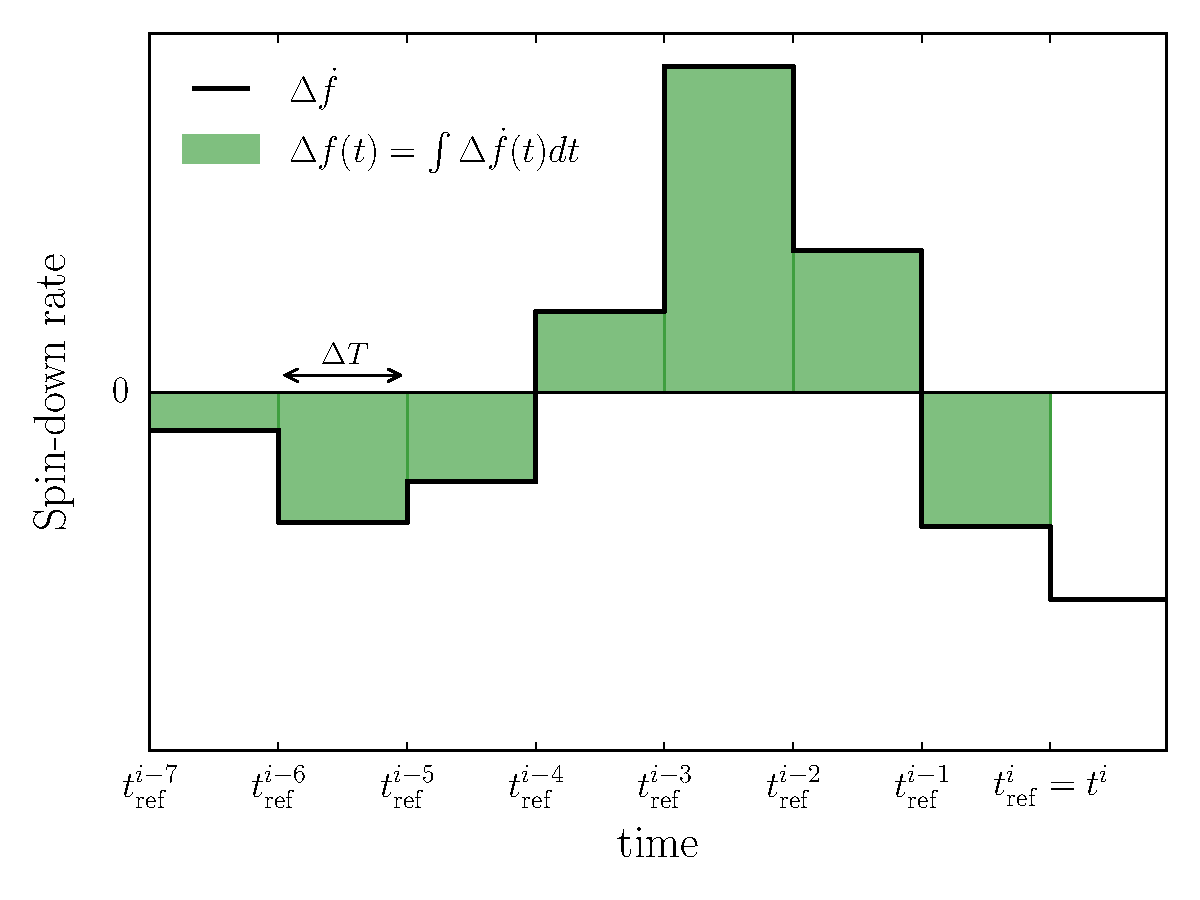
\includegraphics[width=0.7\textwidth]{Illustration_F1_int}
\caption{An example of a random walk in the spin-down rate,
Eqn.~\eqref{eqn: delta fdot n}. The filled green blocks indicate the
summation defined in Eqn.~\eqref{eqn: f offset induced} required to
calculate the induced change in frequency at $t^{i}$ due to the random walk in
spin-down rate.}
\label{fig: Illustration fdot int}
\end{figure}

If we want to model a random walk in the phase, frequency, and spin-down rate
concurrently, then we must consider the effect that a
random walk in spin-down will have on the frequency and phase. For example, if we
increase the spin-down rate for a period of time, then we would expect the frequency
to decrease at a greater rate during this period. In our discrete model, it is
not possible to dynamically change the frequency during a single subdomain.
However, we can approximate this by updating the frequency in the next
subdomain with the induced frequency offset due to the spin-down in all the previous
subdomains. This must be done for the induced effect from the random walk in spin-down rate on
the phase and frequency, and for the induced effect from the random walk in frequency
on the phase. There is no induced effect for the spin-down rate: the effect only
propagates to lower order terms.

Because the random walk is discrete and modelled as constant in any given
subdomain, we can calculate the offset in the lower order terms from a Taylor
expansion. The total offset at the  $i^{th}$ reference time is then given by
the summation of the offset caused by all higher order terms up to that
reference time. We can choose the reference times arbitrarily, but setting each
to start at the beginning of the subdomain simplifies the calculation.  For the
frequency offset induced by the spin-down, we have
\begin{equation}
\Delta \f_{i} = \s{j=1}{i-1}\Delta\fdot_{j} \dT .
\label{eqn: f offset induced}
\end{equation}
This can be thought of as the integration of the spin-down up to the $i^{th}$
reference time and is illustrated by the green blocks in Figure~\ref{fig:
Illustration fdot int}.

We want to consider random walks in all three parameters so we now add in a
random walk in frequency. Each step is independent of the induced effect from
the spin-down and is given by \mbox{$\tn \f_{i} \sim \mathcal{N}(0, \sigF)$}. The two
effects will sum linearly such that the frequency offset is
\begin{equation}
\Delta \f_{i} = \s{j=1}{i}\tn \f_{j} + \s{j=1}{i-1}\Delta\fdot_{j} \dT.
\label{eqn: f offset}
\end{equation}

By a similar process we can calculate the induced effect of the frequency and
spin-down on the phase. Including the random walk in the phase
for which $\tn \phi_i \sim \mathcal{N}(0, \sigP)$, the phase offset is given by
\begin{equation}
\Delta\phi_{i}  =  \s{j=1}{i}\tn \phi_{j}
+ 2\pi\left(\s{j=1}{i-1}\Delta \f_{j}\dT
+ \frac{1}{2}\s{j=1}{i-1}\Delta \fdot_{j}\dT^{2}\right).
\label{eqn: phi offset}
\end{equation}

%Equations \eqref{eqn: f offset} and \eqref{eqn: phi offset} will allows us to
%construct the parameter space offsets in all three terms from the distibutions
%$\tn \phi_i$, $\tn \phi_i$, and $\tn \phi_i$.
\subsection{Writing the parameter offsets in terms of normal distributions}
Eqn~\eqref{eqn: f offset} and Eqn.~\eqref{eqn: phi offset} give the difference
between the signal and template as
functions of the random walks in higher order parameters. In order to calculate
statistical values, we now write these in terms of the normal distributions
from which the random walks are constructed.  Substituting Eqn.~\eqref{eqn:
delta fdot n} into Eqn.~\eqref{eqn: f offset} and using the identity defined
in Eqn.~\eqref{eqn: SI 1} of Appendix~\ref{sec: summation identities}, we have
\begin{align}
\Delta \f_{i}  & = \s{j=1}{i}\tn \f_{j}
+ \s{j=1}{i-1}\s{k=1}{j}\tn \fdot_{k} \dT ,  \\
& = \s{j=1}{i}\tn \f_{j}
+ \s{j=1}{i-1}(i-j)\tn \fdot_{j} \dT .
\label{eqn: delta f n}
\end{align}
Similarly, substituting this equation into Eqn.~\eqref{eqn: phi offset} and
using both Eqn.~\eqref{eqn: SI 1} and Eqn.~\eqref{eqn: SI 2} from
Appendix~\ref{sec: summation identities}, we have
\begin{align}
\begin{split}
\Delta\phi_{i} & = \s{j=1}{i}\tn \phi_{j}
+ 2\pi \left(\s{j=1}{i-1}\Delta\f_{j}\dT
+ \frac{1}{2}\s{j=1}{i-1}\Delta\fdot_{j}\dT^{2}\right) \\
& = \s{j=1}{i}\tn \phi_{j} + 2\pi\left(\s{j=1}{i-1}\left(\s{k=1}{j}\tn\f_{k}
+ \s{k=1}{j-1}(j-k)\tn\fdot_{k}\dT\right)\dT
 + \frac{1}{2}\s{j=1}{i-1}\s{k=1}{j}\Delta\fdot_{k}\dT^{2} \right)  \\
& = \s{j=1}{i}\tn \phi_{j} + 2\pi\left(\s{j=1}{i-1}(i-j)\tn\f_{j}\dT
 + \s{j=1}{i-1}\s{k=1}{j-1}(j-k)\tn\fdot_{k}\dT^{2}
 + \frac{1}{2}\s{j=1}{i-1}(i-j)\Delta\fdot_{j}\dT^{2} \right)  \\
& = \s{j=1}{i}\tn \phi_{j} + 2\pi\left(\s{j=1}{i-1}(i-j)\tn\f_{j}\dT
 + \frac{1}{2}\s{j=1}{i-1}\left(\left(i-j\right)\left(i-j-1)\right)
 + (i-j)\right)\tn\fdot_{j}\dT^{2}\right)  \\
& = \s{j=1}{i}\tn \phi_{j} + 2\pi\left(\s{j=1}{i-1}(i-j)\tn\f_{j}\dT
 + \frac{1}{2}\s{j=1}{i-1}(i-j)^{2}\tn\fdot_{j}\dT^{2}\right).
\end{split}
\label{eqn: delta phi n}
\end{align}
This result can be interpreted as the accumulated phase over a time $i\Delta
T$ due to a random walk in the phase, frequency, and spin-down rate.



\section{Random walk models: a simple treatment}
\label{sec: random walk models part I}
We will now calculate the mismatch for a fully-coherent search given the
random walk in phase, frequency, and spin-down rate defined in the previous
section.

Let us begin by expanding the metric-mismatch summation from Eqn.~\eqref{eqn:
mismatch}. Recalling that Greek indices label the parameter components and
Roman indices label the subdomain, then writing the summations explicitly, we
have
\begin{align}
\mutilde & = g_{\alpha\beta i j}\dl^{\alpha i}\dl^{\beta j}  \\
&=\s{i=1}{\Nsd}\s{j=1}{\Nsd}g_{\alpha\beta i j}\dl^{\alpha i}\dl^{\beta j}  \\
&= \s{i=1}{\Nsd}g_{\alpha\beta i i}\dl^{\alpha i}\dl^{\beta i}
+ \s{i=1}{\Nsd} \s{\substack{j=1\\ j \ne i}}{\Nsd} g_{\alpha \beta ij}\dl^{\alpha i}\dl^{\beta j}.
\end{align}
The summation has been intentionally split into terms for which the two
subdomains are the same and those for which they are different. We calculated
the metric when the reference time is at the beginning of each subdomain in
Eqn.~\eqref{eqn: metric equal subdomains tref 0}; by considering this metric for
the two cases, we can define two distinct components as
\begin{equation}
g_{\alpha\beta ij} = \left\{
\begin{array}{cc}
g_{\alpha\beta}^{\mathrm{E}} & \textrm{ if } i =j \\
g_{\alpha\beta}^{\mathrm{NE}} & \textrm{ if } i  \ne j
\end{array}\right.  .
\end{equation}
Finally, we can calculate the fully-coherent metric-mismatch from
\begin{align}
\mutilde &= \s{i=1}{\Nsd}g_{\alpha\beta}^{\mathrm{E}}\dl^{\alpha i}\dl^{\beta i}
+ 2\s{i=1}{\Nsd} \s{j=1}{i-1} g_{\alpha \beta}^{\mathrm{NE}}\dl^{\alpha i}\dl^{\beta j} .
\label{eqn: mismatch sep}
\end{align}

\subsection{Taking the expectation}

In Eqn.~\eqref{eqn: delta fdot n}, Eqn.~\eqref{eqn: delta f n},
Eqn.~\eqref{eqn: delta phi n} we have written the parameter space offsets
(which are to be used in calculating the mismatch) purely in terms of the
random walk distributions $\tn \phi_i$, $\tn \f_i$, and $\tn \fdot_i$. We can
calculate the mismatch exactly given a set of random walk jumps by inserting
these into Eqn.~\eqref{eqn: mismatch sep}. However, since we are dealing with
statistical quantities, we can instead infer the behaviour of the mismatch
under the random walk by taking an expectation.

Inserting Eqn.~\eqref{eqn: delta fdot n}, Eqn.~\eqref{eqn: delta f n},
Eqn.~\eqref{eqn: delta phi n}  in Eqn.~\eqref{eqn: mismatch sep} yields a
number of terms with all the permutations of two terms from $[\tn \phi, \tn \f,
\tn \fdot]$. Taking the expectation, all the cross-correlated terms, such as
$\tn\phi_{i}\tn \fdot$, will have an expectation of zero since the steps of the
random walk are independent. The only non-vanishing terms are given by
\begin{align}
E[\tn\phi_{i}\tn\phi_{j}] &= \delta_{ij}\sigP, &
E[\tn\f_{i}\tn\f_{j}] &= \delta_{ij}\sigF,&
E[\tn\fdot_{i}\tn\fdot_{j}] &= \delta_{ij}\sigS,
\end{align}
After some simplification we find that the mismatch is given by
\begin{align}
\begin{split}
E[\mutilde]   = &  \frac{A_{\phi}}{6} \left(\Nsd - \frac{1}{\Nsd}\right)
+ \frac{\pi^{2} A_{{f}}}{30}\left(4 \Nsd^{3} + 5 \Nsd^{2} + \frac{1}{\Nsd}\right)\\
 & +  \frac{\pi^{2} A_{{\dot{f}}}}{3780} \left(66 \Nsd^{5} - 21 \Nsd^{3} + 105 \Nsd^{2}
 + 217 \Nsd + 63 - \frac{94}{\Nsd}\right),
\end{split}
\label{eqn: expectation}
\end{align}
where
\begin{equation}
	A_{\phi} = \sigP \;\;\;\;\;
    A_{\f} = \sigF\Delta T^{2} \;\;\;\;\;
    A_{\fdot} = \sigS\Delta T^{4},
\end{equation}
define three dimensionless `activity parameters'.

Recalling that $\Nsd=\Tobs/\Delta T$, Eqn.~\eqref{eqn: expectation} makes
predictions for the leading order
scaling of the three random walks with the observation period
\begin{equation}
E[\mutilde]_{\mathrm{PN}} \sim \sigP \frac{\Tobs}{\Delta T}, \hspace{10mm}
E[\mutilde]_{\mathrm{FN}} \sim \sigF \frac{\Tobs^{3}}{\Delta T}, \hspace{10mm}
E[\mutilde]_{\mathrm{SN}} \sim \sigS \frac{\Tobs^{5}}{\Delta T}.
\label{eqn: scalings}
\end{equation}
We note here the exact relation to the scaling of the variance of the
root-mean phase residual as calculated by \citet{Cordes1980} and given in
Eqn.~\eqref{eqn: S calc}. We will return to this later in Sec.~\ref{sec: understanding the random walk model}.

\subsection{Verifying the results}
\label{sec: verifying}

We can observe the leading order scaling of Eqn.~\eqref{eqn: scalings} directly
and verify the predictions made by Eqn.~\eqref{eqn: expectation} by comparing
with exact numerical results. That is, using the \verb+LALSuite+
\cite{lalsuite}  signal injection and recovery tools developed in
Section~\ref{sec: narrow-band method} of Chapter~\ref{sec: timing noise in
cgw} we simulate signals undergoing a random walk and calculate the
corresponding mismatch (no minimisation step is done here, this is discussed in
the next section). In particular, we perform three Monte Carlo studies for a
random walk in the phase, frequency, and spin-down rate and in each case
compare the simulated results with the analytic prediction. The results are
shown in Figure~\ref{fig: rw I} and demonstrate good agreement between the
simulation means and the prediction of Eqn.~\eqref{eqn: expectation}.

\begin{figure}[ht]
\centering
\subfloat[Random walk in phase]{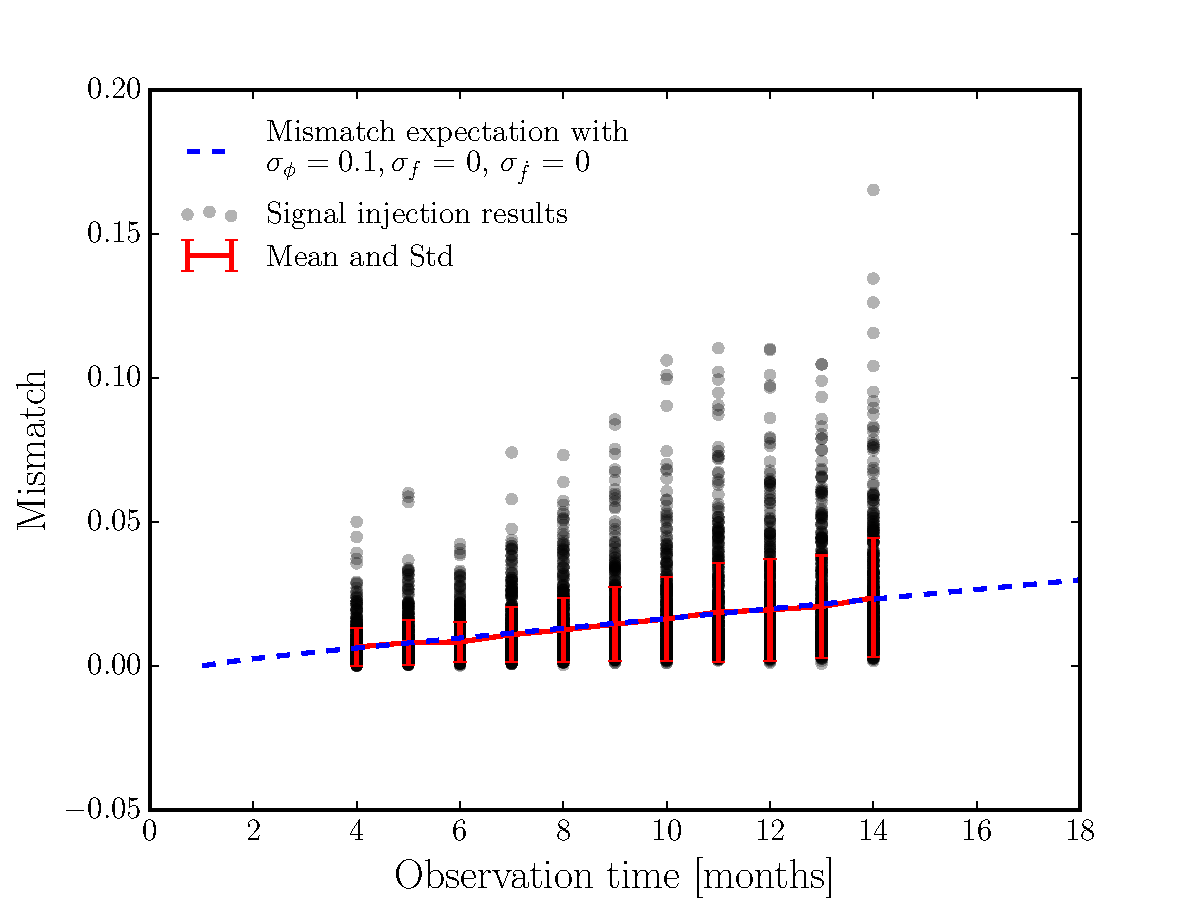
\includegraphics[width=0.5\textwidth]{ExpectationPhase}}
\subfloat[Random walk in frequency]{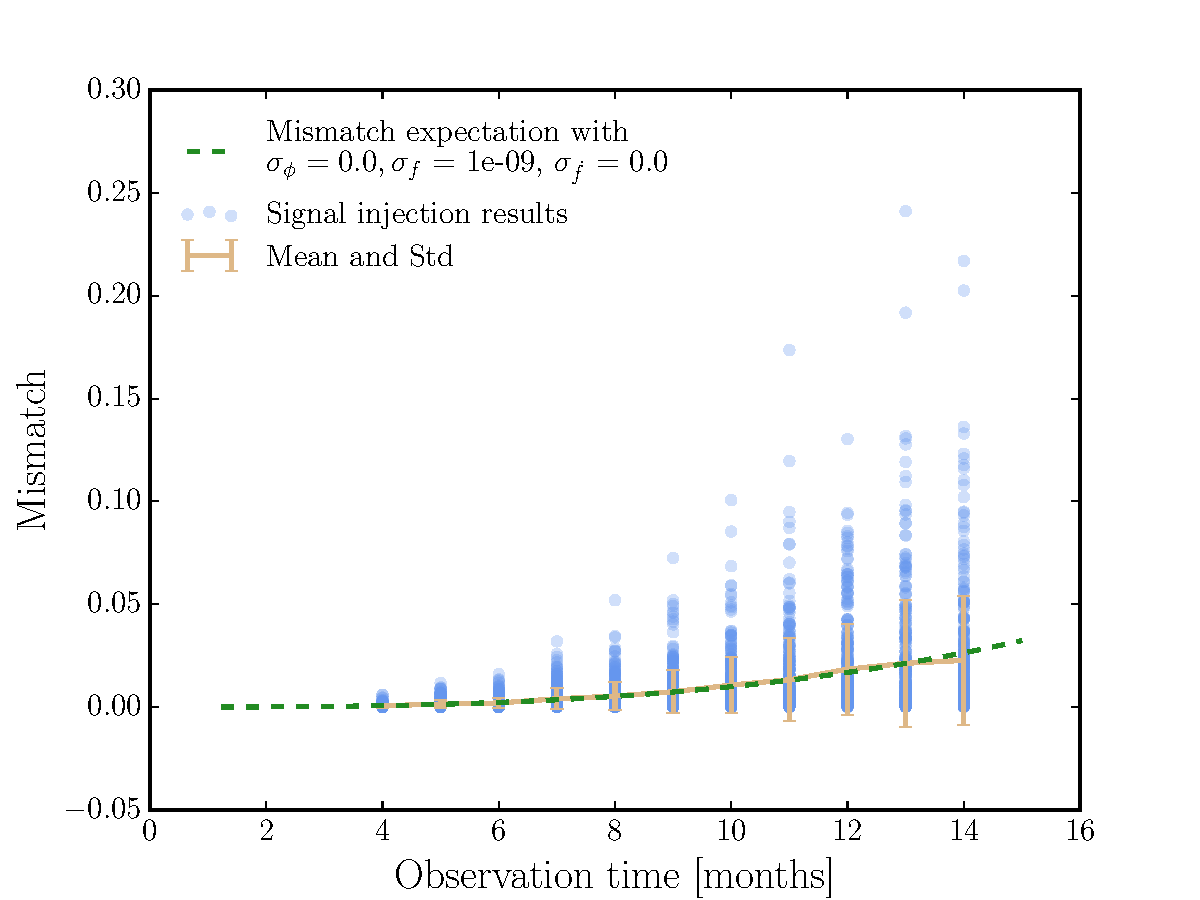
\includegraphics[width=0.5\textwidth]{ExpectationFrequency}}\\ \subfloat[Random walk in spin-down]{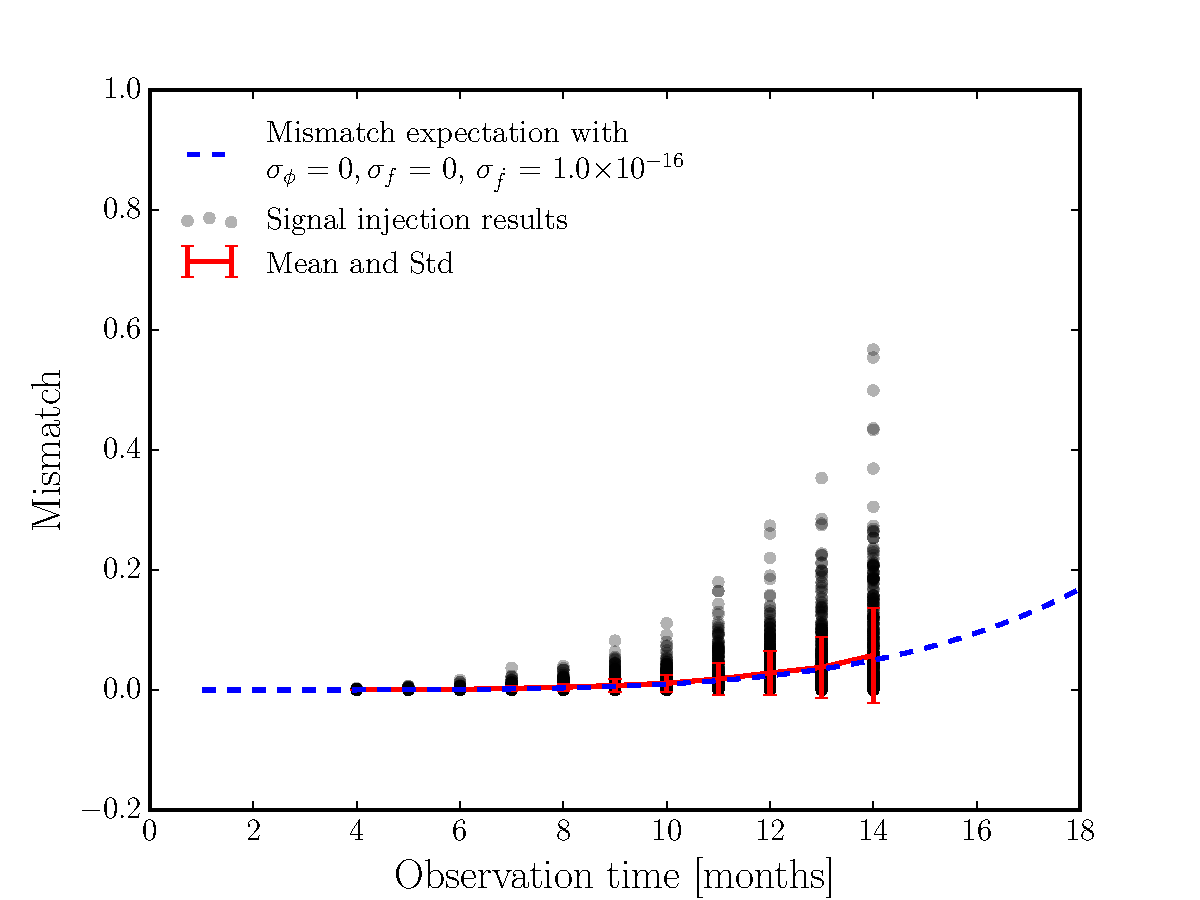
\includegraphics[width=0.5\textwidth]{ExpectationSpindown}}
\caption{A comparison of Monte Carlo numerical simulated mismatch with the prediction
of Eqn.~\eqref{eqn: expectation} for a random walk in the phase, frequency,
and spin-down rate.}
\label{fig: rw I}
\end{figure}

\section{Random walk models: minimising the mismatch}
\label{sec: random walk models part II}
In Section~\ref{sec: defining a random walk} we have defined a random walk
model for which we subsequently calculated the fully-coherent mismatch in
Section~\ref{sec: random walk models part I}. However, this is a special case
in which the random walk for each parameter offset (the difference between the
signal and the template) begins at the origin and then grows with time. It is
the signal which undergoes a random walk, so in this case we have set the
template to exactly match the signal at~$t=0$. However, one could imagine choosing
a different template which would reduce the overall mismatch; as such
Eqn.~\eqref{eqn: expectation} may overestimate the mismatch. The proper thing to
do is to minimise the mismatch with respect to the
template parameters~$\lt^{\alpha}$ which are implicitly in the calculation of
Section~\ref{sec: random walk models part I} through the parameter space
offset
\begin{align}
\Delta \lambda^{\alpha i} = \ls^{\alpha i} - \lt^{\alpha i},
\end{align}
as first defined in Section~\ref{sec: generalising the metric-mismatch}.

Ideally, we would like to repeat the calculation leading to Eqn.~\eqref{eqn:
expectation} minimising the mismatch with respect to the template parameters.
However, this calculation is difficult and so we have not yet attempted it.  A
practical alternative method which we will use here is to begin with the random
walk starting at the origin, as defined in Section~\ref{sec: defining a random
walk}, and then fit a polynomial of degree $k$ minimising the root-mean-square
residual between the parameter space offset and the polynomial. We then
subtract the best-fit polynomial from the parameter space offset, this leaves
us with a residual parameter space offset for which we then compute the
mismatch. We will verify that this captures the essential features of
minimising the mismatch by comparing with numerical simulations in which the
exact mismatch is minimised numerically.

In Appendix~\ref{sec: least squares minimisation of a random walk}, we
introduce the basic tools of least squares fitting and removing a polynomial of
degree $k$ to a generic random walk. In the following sections, we will
calculate the minimised mismatch for random walks in the phase or frequency; we
have not yet calculated the corresponding result for mixtures or random walks
in the spin-down rate. In this process, we have a choice in the degree of
polynomial to fit and remove. Since most searches minimise the mismatch with
respect to the template frequency $f_\textrm{t}$ and spin-down rate
$\dot{f}_{\textrm{t}}$, this is equivalent to fitting and removing a $k=2$
polynomial to the phase residual. In the following sections we will first
calculate the analytic results and then verify that these agree with exact
numerical results in Section~\ref{sec: verifying minimised}.

\subsection{Random walk in the phase}
\label{sec: minimised rw in phase}
We begin with the simplest case of a random walk in phase, for which we have
\begin{equation}
\Delta\phi_{i} = \s{j=1}{i}\mathcal{N}(0, \sigP).
\end{equation}
Then, as shown in Eqn.~\eqref{eqn: E yiyi} of Appendix~\ref{sec: least squares
minimisation of a random walk}, we have that
\begin{equation}
E[\Delta\phi_{i} \Delta\phi_{j}] = \sigP \min(i, j).
\end{equation}

We define the residual difference between the signal and template
after fitting and removing the best-fit $2^{nd}$ order polynomial, $\hat{y}_i^{(2)}$, as
\begin{align}
\Delta^{(2)}\phi_i = \Delta\phi_i - \hat{y}_i^{(2)}.
\label{eqn: D2phi}
\end{align}
Note that the superscript `(2)' indicates the degree of polynomial and by
$\Delta^{(2)}\phi_i$ we mean the residual difference between the signal and
template after fitting and removing the polynomial.

We set the difference between the signal and template in all other parameters
to zero such that the mismatch for a random walk in the residual phase is
therefore
\begin{align}
\mutilde & = g_{0 0 i j} \Delta^{(2)}\phi^{i}\Delta^{(2)}\phi^{j} \\
& = \s{i=1}{\Nsd}g_{00}^{E} \Delta^{(2)}\phi_{i}\Delta^{(2)}\phi_{i}
+ 2 \s{i=1}{\Nsd}\s{j=1}{i-1}g_{00}^{NE}\Delta^{(2)}\phi_{i}\Delta^{(2)}\phi_{j}.
\label{eqn: 4202540871}
\end{align}
To calculate the expectation of the mismatch, we need to evaluate the
expectation of
\begin{align}
\Delta^{(2)}\phi_{i}\Delta^{(2)}\phi_{j} = & \left(\Delta\phi_{i}
- \s{k=1}{\Nsd}\CT_{ik}\Delta\phi_{k}\right)
 \left(\Delta\phi_{j} - \s{l=1}{\Nsd}\CT_{jl}\Delta\phi_{l}\right) \\
= & \Delta\phi_{i}\Delta\phi_{j} -
\left(\s{k=1}{\Nsd}\CT_{ik} \Delta\phi_{j}\Delta\phi_{k}
+ \s{l=1}{\Nsd}\CT_{jl}\Delta\phi_{i}\Delta\phi_{l}\right) \nonumber \\
& +
\s{k=1}{\Nsd}\s{l=1}{\Nsd}\CT_{ik}\CT_{jl} \Delta\phi_{k}\Delta\phi_{l},
\end{align}
where $\CT_{ij}$ is defined in Eqn.~\ref{eqn: C_2} and Eqn.~\ref{eqn: MC_2} of
Appendix~\ref{sec: least squares minimisation of a random walk} and we have
replaced the $\Delta x$ notation of the appendix with the time $\dT$. Then
taking the expectation
\begin{align}
\E{\Delta^{(2)}\phi_{i}\Delta^{(2)}\phi_{j}} & =
%E\left[\Delta\phi_{i}\Delta\phi_{j}\right] -
%\left(\s{k=1}{\Nsd}E[\Delta\phi_{j}\Delta\phi_{k}]
%+ \s{l=1}{\Nsd}E[\Delta\phi_{i}\Delta\phi_{l}]\right) +
%\s{k=1}{\Nsd}\s{l=1}{\Nsd}E[\Delta\phi_{k}\Delta\phi_{l}]\\
%& =
\sigma^{2}_{\phi} \left(\min(i, j) - \left(\s{k=1}{\Nsd}\CT_{ik} \min(j, k)
+ \s{l=1}{\Nsd}\CT_{jl}\min(i, l) \right)\right. \notag \\
& \hspace{13mm} \left. + \s{k=1}{\Nsd}\s{l=1}{\Nsd}\CT_{ik}\CT_{jl}\min(k, l)\right).
\label{eqn: expected mismatch dP0idP0j_k2}
\end{align}
Using symbolic mathematics packages we
calculate an analytic expression which is a function of $\dT, i, j$ and $\Nsd$.
Inserting this into Eqn.~\eqref{eqn: 4202540871} and simplifying we find that
\begin{align}
E[\mutilde]  & = \s{i=1}{\Nsd}g_{00}^{E} E\left[\Delta^{(2)}\phi_{i}\Delta^{(2)}\phi_{i}\right]
+ 2 \s{i=1}{\Nsd}\s{j=1}{i-1}g_{00}^{NE}E\left[\Delta^{(2)}\phi_{i}\Delta^{(2)}\phi_{j}\right]  \\
& = \frac{1}{70}\sigP\left(3N - \frac{27}{\Nsd}\right).
\label{eqn: Expected mismatch RW in phase k2}
\end{align}
This expression can be compared to Eqn.~\eqref{eqn: expectation} ignoring the
effect of the random walk in the frequency and spin-down rate. Notably, we
retain the same leading order scaling of $\Nsd$, but the overall coefficient is
decreased; the same effect was found by \citet{Cordes1980} for the
root-mean-square phase residual after removing a polynomial.

Rearranging the expression in the bracket demonstrates the mismatch is negative
or zero for $1 \ge \Nsd \ge 3$. This is a reflection of the minimum number of
points needed in order to perform the quadratic fit. We will discuss this in more
detail in Sec.~\ref{sec: appendix conclusions} for the simpler case of fitting
and removing a polynomial from a generic random walk.

\subsection{Random walk in the frequency}

For a random walk in the frequency we have an added complexity caused by the
effect the frequency offsets induces in the phase. For the frequency offset, we
have
\begin{align}
\Delta f_{i} &= \s{j=1}{i}\mathcal{N}(0, \sigF).
\end{align}
Recalling that we set the reference time at the beginning of each subdomain,
then as in Section~\ref{sec: defining a random walk}, the induced phase offset is
\begin{align}
\Delta\phi_{i} &=2\pi \s{j=1}{i-1}\Delta f_{j}\dT \\
 & = 2\pi\dT \s{j=1}{i-1}\s{k=1}{j}\mathcal{N}(0, \sigF) \\
& = 2\pi\dT \s{j=1}{i}(i-j)\mathcal{N}(0, \sigF).
\label{eqn: P2F}
\end{align}
Note that we do not include a random walk in the phase here.

Then we calculate the expected values of combinations of the parameter space
offsets using Eqn.~\eqref{eqn: E yiyi} from Appendix~\ref{sec: least squares
minimisation of a random walk} and the two summation identities
Eqn.~\eqref{eqn: SI 1} and Eqn.~\eqref{eqn: SI 2} from Appendix~\ref{sec:
summation identities}, this gives
\begin{align}
E[\Delta\f_{i}\Delta\f_{j}] & = \sigF \min(i, j), \label{eqn: E1} \\
E[\Delta\phi_{i}\Delta\f_{j}] & = 2 \pi \dT \sigF \s{k=1}{\min(i, j)}(i-k), \label{eqn: E2}\\
E[\Delta\phi_{i}\Delta\phi_{j}] & =
\left(2\pi\dT\right)^{2}\sigF \s{k=1}{\min(i, j)}(i-k)(j-k).
\label{eqn: E3}
\end{align}

In Eqn.~\eqref{eqn: D2phi}, we defined the residual difference between the signal
and template phase after fitting and removing a second order polynomial. The
second order polynomial was chosen to model the effect of minimising over the
template frequency and frequency derivative. Let us now define
\begin{align}
\Delta^{(1)}f_i = \Delta f_i - \hat{y}^{(1)}_i,
\label{eqn: D2f}
\end{align}
as the residual difference between the signal and template frequency after
fitting and removing a first order polynomial. In this instance, the first
order polynomial models the effect of minimising over the template
frequency and frequency derivative.

To calculate the mismatch, we expand Eqn.~\eqref{eqn: mismatch} summing over
the residual frequency offset $\Delta^{(1)}f_i$ (defined in Eqn.~\eqref{eqn:
D2f}) and the residual phase offset $\Delta^{(2)}\phi_i$ (given by
substituting Eqn.~\eqref{eqn: P2F} into Eqn.~\eqref{eqn: D2phi}), this gives
\begin{align}
\begin{split}
E[\mutilde] = &
\s{i=1}{\Nsd}\left(g_{00}^{E}E\left[\Delta^{(2)}\phi_{i}\Delta^{(2)}\phi_{i}\right]
+ 2 g_{01}^{E}E\left[\Delta^{(2)}\phi_{i}\Delta^{(1)}\f_{i}\right]
+  g_{11}^{E} E\left[\Delta^{(2)}\f_{i}\Delta^{(1)}\f_{i}\right] \right) \\
& + 2\s{i=1}{\Nsd}\s{j=1}{i-1}\left(\right.
g_{00}^{NE}E\left[\Delta^{(2)}\phi_{i}\Delta^{(2)}\phi_{j}\right] +
g_{01}^{NE}E\left[\Delta^{(2)}\phi_{j}\Delta^{(2)}\f_{i}\right] +  \\
&\hspace{20mm}\left. g_{10}^{NE}E\left[\Delta^{(2)}\phi_{i}\Delta^{(2)}\f_{j}\right] +
g_{11}^{NE} E\left[\Delta^{(1)}\f_{i}\Delta^{(1)}\f_{j}\right] \right).
\end{split}
\end{align}


We calculate each of these expressions in a similar manner to Eqn.~\eqref{eqn:
expected mismatch dP0idP0j_k2} replacing the relevant expectations with those
given in Eqn.~\eqref{eqn: E1} to Eqn.~\eqref{eqn: E3}. This yields an expected
mismatch given by
\begin{equation}
E[\mutilde] = \frac{\pi^{2} }{630} \sigF \dT^{2}  \left(\Nsd^{3} + 13\Nsd + \frac{82}{\Nsd} \right).
\label{eqn: Expected mismatch RW in frequency k2}
\end{equation}
This can be compared with the frequency noise term alone in Eqn.~\eqref{eqn:
expectation}. We note that the leading order power remains unchanged, but there
is a reduction in the coefficient and a difference in the second highest
power. The reduction in the coefficient is expected since we have minimised
the mismatch; we do not have an intuitive explanation for the change in the
second highest power.

\subsection{Verifying the results}
\label{sec: verifying minimised}

We now verify Eqn.~\eqref{eqn: Expected mismatch RW in frequency k2} and
Eqn.~\eqref{eqn: Expected mismatch RW in phase k2} by comparing with Monte
Carlo simulations as we first did in Section~\ref{sec: verifying}. The
numerical signals undergo a random walk as described in Section~\ref{sec:
random walk models part I}, however, when searching for the signals we now search
over a grid of points in $f_\textrm{t}$ and $\dot{f}_\textrm{t}$, then we
select the grid point with the minimum mismatch; this minimises the mismatch
over the frequency and spin-down. The results are plotted in Figure~\ref{fig:
verification of minimised RW} and demonstrate good agreement between the
analytic prediction and the mean of the simulated mismatches.

\begin{figure}[ht]
\centering
\subfloat[Random walk in phase]{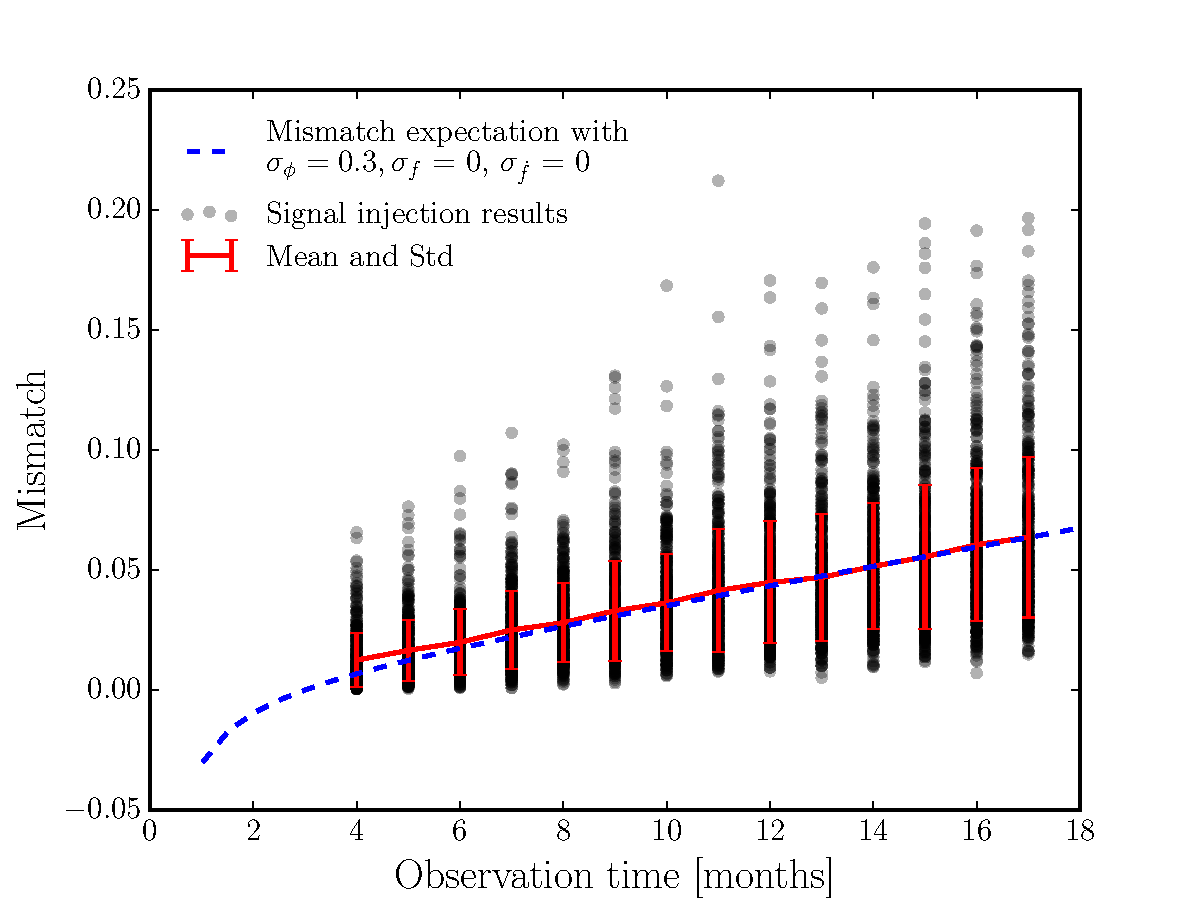
\includegraphics[width=0.5\textwidth]{ExpectationPhase_NarrowBand}}
\subfloat[Random walk in frequency]{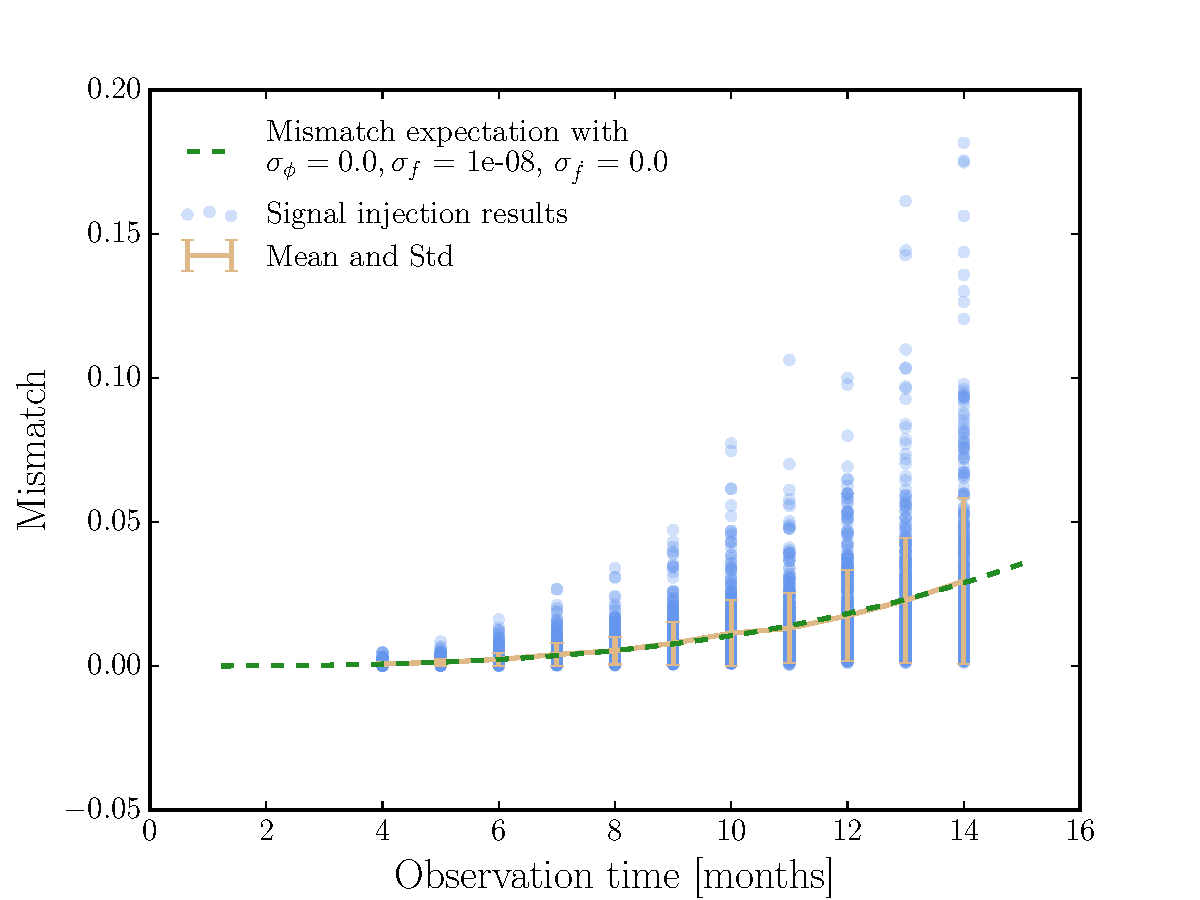
\includegraphics[width=0.5\textwidth]{ExpectationFrequency_NarrowBand}}\\
%\subfloat[Random walk in spin-down]{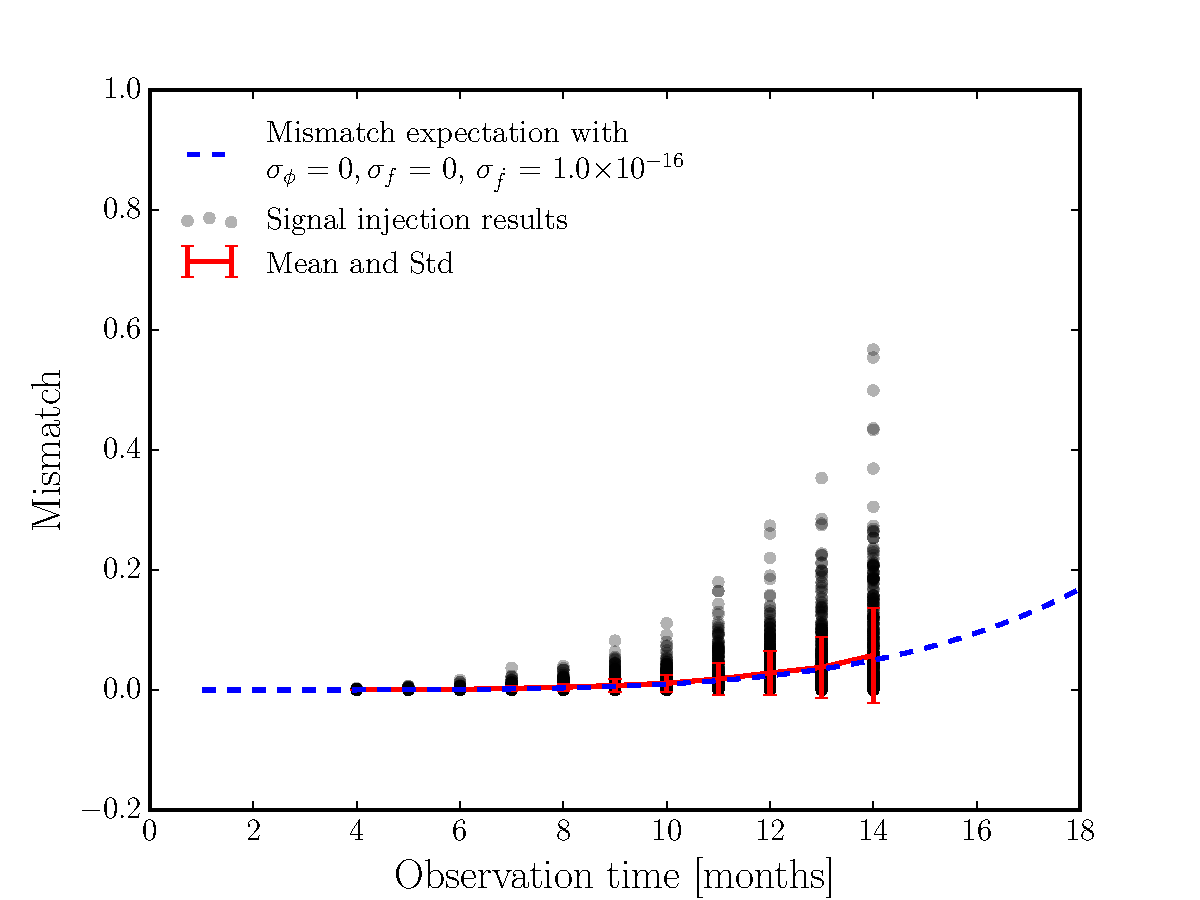
\includegraphics[width=0.5\textwidth]{ExpectationSpindown}}
\caption{A comparison of the Monte Carlo numerical simulated mismatch with the
predictions of Eqn.~\eqref{eqn: Expected mismatch RW in
frequency k2} and Eqn.~\eqref{eqn: Expected mismatch RW in phase k2}; this differs
from Figure~\ref{fig: rw I} in that the numerical mismatch is minimised by selecting
the smallest mismatch from a grid of points in $f_\textrm{t}$ and $\dot{f}_\textrm{t}$.}
\label{fig: verification of minimised RW}
\end{figure}

\section{Understanding the random walk model}
\label{sec: understanding the random walk model}

In the previous two sections, we have used the random walk model
defined in Section~\ref{sec: defining a random walk} which appears at first to
be non-physical: the random walk `jumps' every $\dT$, but what
physics determines this length? Furthermore, we assumed that the jumps between
adjacent steps (see for example Eqn.~\eqref{eqn: fdot N}) were normally
distributed with zero mean and variance $\sigP, \sigF$, and $\sigS$, but how
physical is this assumption?
In this section, we will show that such a
random walk is equivalent to the more natural `compound Poisson random walk
process' introduced in Section~\ref{sec: TN interpretations random walk models}
which is used in the literature to model timing noise as a random walk.  The
methods discussed here parallel the work of \citet{Cordes1980} and
\citet{Groth1975}, but are described in detail as there are some subtleties to
our analysis.

Consider a parameter $\Delta X(t) \in [\Delta\phi, \Delta\nu,\Delta\dot{\nu}]$ being
the difference between the real noisy signal and the search template. $\Delta
X(t)$ then encodes the deviations due to timing noise without concerning the
secular spin-down.  We will model timing noise by allowing $\Delta X(t)$ to
undergo a \emph{compound Poisson process}: a random walk where events are
Poisson distributed in time occurring with a rate $\lambda$, but the size the
events are drawn from a normal distribution with zero mean and a variance
$\langle \delta X^{2} \rangle$, or more formally
\begin{align}
\Delta X(t) = \sum_{i=1}^{N(t)} \delta X_i,
\label{eqn: X def}
\end{align}
where $\{ N(t): t \ge 0\}$ is a Poisson process with rate $\lambda$ and
$\{\delta X_i: i \ge 1\}$ are independent and identically distributed with
$\delta X_i \sim N(0, \langle \delta X^{2}\rangle)$. Note that $\langle \delta X^{2} \rangle$
where $X \in [\phi, \nu, \dot{\nu}]$ is the variance of the random walk jumps.

If the event rate $\lambda$ of the compound Poisson process is sufficiently
large such that in a time $\dT$ the number of events is large, it can be shown
that, due to the central limit theorem
(see for example \citet{weiss2006course}), $\Delta X_i(\dT)$ is normally
distributed. The mean can be calculated using Wald's
Eqn.~\citep{wald1944cumulative} which gives
\begin{align}
\langle \Delta X(\dT) \rangle = 0,
\label{eqn: DX mean}
\end{align}
while the variance can be calculated using the law of total variance
\citep{weiss2006course} from which we find that
\begin{align}
\langle \Delta X(\dT)^{2} \rangle &  = \lambda \dT \langle \delta X^{2}\rangle.
\label{eqn: DX var}
\end{align}

If we label the parameter offset measured for blocks of data $\dT$ as  $\Delta
X_{i}(\dT)$ then $\{\Delta X_{1}(\dT), \Delta X_{2}(\dT), \dots\}$ is a
sequence of independent and identically distributed random variables with a mean
and variance given by Eqn.~\eqref{eqn: DX mean} and Eqn.~\eqref{eqn: DX var}
respectively.

In the model defined in Section~\ref{sec: defining a random walk}, we defined
\begin{align}
\tn X_{i} = \Delta X_{i} - \Delta X_{i-1},
\end{align}
as the difference between two adjacent subdomains of the piecewise Taylor
expansion. Moreover, we assumed that $\tn X_i(\dT)$ was normally distributed
with zero mean and a variance $\sigma_{X}^{2}$.  This assumption is valid if
the underlying random walk process is a compound Poisson process. To see this,
we note that if both $\Delta X_{i}$ and $\Delta X_{i-1}$ can be described by
the compound Poisson process in Eqn.~\eqref{eqn: X def} and the assumption of
a large number of events in each is valid, then
\begin{align}
\tn X_{i}(\dT) =  \Delta X_{i}\left(\frac{\dT}{2}\right)
                - \Delta X_{i-1}\left(\frac{\dT}{2}\right),
\end{align}
is the difference between normally distributed random variables. The factors of
a half are due to splitting the period of $\tn X_i(\Delta T)$ into two equal
durations. It can be shown (see for example \citeauthor{wolframdifference})
that the difference between two normal distributions, i.e. $\tn X_i (\dT)$, is
also normally distributed with a mean which is the difference in the means of
$\Delta X_{i}(\dT)$ and $\Delta X_{i-1}(\dT)$:
\begin{align}
\langle \tn X(\dT) \rangle & = 0,
\label{eqn: Poisson expectation}
\end{align}
and a variance which is the sum of the variance of
$\Delta X_{i}(\dT)$ and $\Delta X_{i-1}(\dT)$:
\begin{align}
\langle \tn X(\dT)^{2} \rangle &  =
2 \lambda \frac{\dT}{2} \langle \delta X^{2}\rangle
= \lambda \dT \langle \delta X^{2}\rangle,
\label{eqn: Poisson variance}
\end{align}

The metric-mismatch calculations derived in the previous two sections are
written as a function of $\sigma_{X}^{2} \in [\sigP, \sigF, \sigS]$
which is the variance of $\tn X(\dT)$. We can therefore relate the two by
\begin{align}
\lambda \dT \langle \delta X^{2}\rangle = \sigma_{X}^{2}.
\end{align}
Rearranging this equation, we can equate $\lambda \langle \delta X^2\rangle$ with
a \emph{GW random walk strength parameter} which we define as
\begin{align}
S_{\mathrm{GWPN}} & \coloneqq \lambda \langle \delta \phi^{2} \rangle =
\frac{\sigP}{\dT}, \label{eqn: SPN 2}\\
S_{\mathrm{GWFN}} & \coloneqq \lambda \langle \delta f^{2} \rangle =
\frac{\sigF}{\dT}, \label{eqn: SFN 2}\\
S_{\mathrm{GWSN}} & \coloneqq \lambda \langle \delta \dot{f}^{2} \rangle =
\frac{\sigS}{\dT}.  \label{eqn: SSN 2}
\end{align}

We distinguish between the strength of gravitational wave noise
($S_{\textrm{GWPN}}, S_{\textrm{GWFN}}$ and $S_{\textrm{GWSN}}$) and the usual
strength of noise in the rotational parameters ($S_{\textrm{PN}},
S_{\textrm{FN}}$ and $S_{\textrm{PN}}$) defined in Eqn.~\eqref{eqn: SPN def} to
Eqn.~\eqref{eqn: SSN def}. To relate between these we need to define the
mechanism of gravitational wave emission. In the canonical non-axisymmetric
distortion mechanism, $f = 2\nu$, therefore the underlying jumps in signals are
related by
\begin{align}
\delta \phi & = 2\delta \varphi, \\
\delta f & = 2\delta\nu, \\
\delta \dot{f}& =2\delta\dot{\nu},
\end{align}
where $\varphi, \nu$ and $\dot{\nu}$ are the rotational phase,
frequency, and spin-down rate. The variances of the GW parameters are related
therefore equal to the variances of the rotational parameters multiplied by a
factor of $4$. Therefore, using the definition the rotation noise strengths from
Eqn.~\eqref{eqn: SPN def} to Eqn.~\eqref{eqn: SSN def}, we see that
\begin{align}
S_{\textrm{GWPN}} = 4S_{\textrm{PN}}, \\
S_{\textrm{GWFN}} = 4S_{\textrm{FN}}, \label{eqn: relation}\\
S_{\textrm{GWSN}} = 4S_{\textrm{SN}}.
\end{align}

We can now write the expectation of the fully-coherent metric-mismatch due to
a random walk in terms of these strength parameters. First, for a random walk
in the phase given by Eqn.~\eqref{eqn: Expected mismatch RW in phase k2} we
take just the leading order term and substitute in Eqn.~\eqref{eqn: SPN 2},
this results in
\begin{align}
\textrm{E}[\mutilde] = \frac{3}{70} S_{\textrm{GWPN}} \Tobs.
\label{eqn: mu prediction phase}
\end{align}
Second, for a random walk in the frequency, we take the leading order terms
from Eqn.~\eqref{eqn: Expected mismatch RW in frequency k2} and substitute
using Eqn.~\eqref{eqn: SFN 2}, this gives
\begin{align}
E[\mutilde] & = \frac{\pi^{2}}{630} S_{\textrm{GWFN}} \Tobs^{3},
\label{eqn: mu prediction}
\end{align}
from this we see how, when the random walk is considered as a compound Poisson
random walk, the mismatch does not depend on $\dT$. The justifies the
random walk treatment that was used in the earlier sections.

\section{Application to the Crab pulsar}
\label{sec: application to the crab}
In Section~\ref{sec: timing noise as described by the crab ephemeris}, we
introduced the Crab ephemeris.  The regular and independent measurements of the
frequency and spin-down rate in the Crab ephemeris provide a unique view of
timing noise as a `jump' in the phase, frequency, and spin-down rate each
month. Specifically by a jump we mean the discontinuity at the interface
between two months as illustrated in Figure~\ref{fig: template jumps}. In this
section, we will interpret data from the ephemeris in the context of a random
walk model. Note that in this section,
we discus the rotational frequency and frequency derivatives, which we denote
by $\nu$ and $\dot{\nu}$ which we will relate to the gravitational wave
frequency $f$ using the non-axisymmetric emission model for which $f=2\nu$.

\subsection{Distribution of jumps in the Crab ephemeris}
\label{sec: jumps}
\newcommand{\nuddotav}{\ddot{\nu}_{\textrm{av}}}
We begin with a purely empirical look at the distribution of jumps in the
Crab ephemeris. We will use the jumps in frequency in the next section to interpret the
Crab ephemeris in the context of a random walk.

From the Crab ephemeris, there are three distributions which we will calculate
here: the jumps in frequency, spin-down rate, and phase. It is not meaningful
to simply look at the difference in frequency (for example) between any two
months without adjusting for the secular spin-down. But what we really want is the
difference which occurs at the interface. To calculate this we define
$\nu_{i}(t)$ as the frequency according to the $i^{th}$ month as evaluated at
time $t$. Then if $\Delta t_{i} = t_{i+1} - t_{i}$ the frequency jump between
months is
\begin{align}
\tn\nu_{i} &= \nu_{i+1}\left(t_{i+1}-\Delta t_{i}/2\right) -  \nu_{i}\left(t_{i}+\Delta t_{i}/2\right), \\
    &= \left[\nu_{i+1}- \frac{\Delta t_{i}}{2}\dot{\nu}_{i+1} + \left(\frac{\Delta t_{i}}{2}\right)^{2}\frac{\ddot{\nu}_{i+1}}{2}\right]
     - \left[\nu_{i} + \frac{\Delta t_{i}}{2}\dot{\nu}_{i}+ \left(\frac{\Delta t_{i}}{2}\right)^{2}\frac{\ddot{\nu}_{i}}{2}\right] .
\end{align}
The Crab ephemeris does not include the second order spin-down, but since the
first order spin-down is not constant we assume a constant average second order
spin-down given by
\begin{equation}
   \nuddotav = \frac{1}{N}\sum_{i} \frac{\dot{\nu}_{i+1} - \dot{\nu_{i}}}{t_{i+1} - t_{i}},
   \label{eqn: average second order spin-down}
\end{equation}
where $N$ is in the number of data points in the ephemeris file. Inserting this
into the Taylor expansion the second order terms cancel leaving a frequency
jump between months given by
\begin{equation}
\tn\nu_{i} = \left(\nu_{i+1}- \nu_{i}\right) -  \left(\dot{\nu}_{i+1}
               + \dot{\nu}_{i}\right)\frac{\Delta t_{i}}{2}.
\label{eqn: crab frequency residuals}
\end{equation}
Note, this is not the difference in frequency between monthly
updates, but the jump between months in frequency at the interface as illustrated in figure
\ref{fig: template jumps}.

Calculating the result of Eqn.~\eqref{eqn: crab frequency residuals} for all
the data points in the Crab ephemeris we plot the estimated density using the
Gaussian kernel density estimate (KDE) method \citep{Scipy} in Figure~\ref{fig:
crab kde}A. Note that we have filtered out differences which occur over known
glitches as described by \citet{Espinoza2011}. This is because we are
interested in the timing noise activity and not the effect of glitches
themselves.
\begin{figure}[ht]
\centering
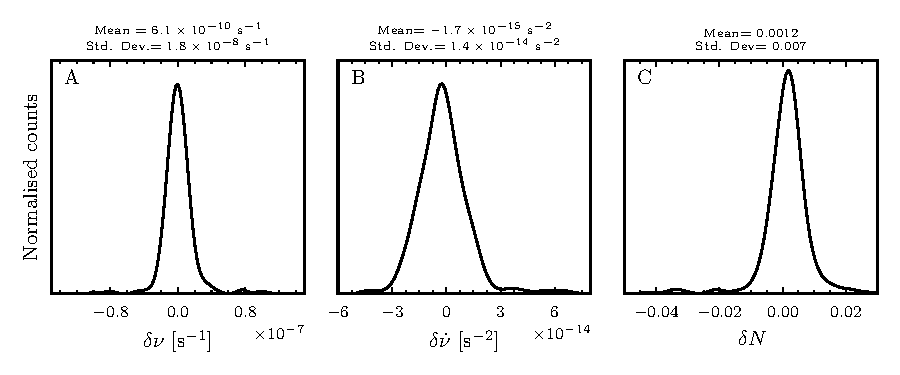
\includegraphics[]{CrabTN_KDEs.pdf}
\caption{KDEs for the `jumps' in frequency, spin-down rate, and residual number
of rotations between adjacent per-month signals in the Crab ephemeris.
Adjacent signals over glitches are filtered along with large anomalous values
of $\tn N$ once it was confirmed they occur within 200 days after a glitch.}
\label{fig: crab kde}
\end{figure}

Moving now to the spin-down, we can calculate the jump between months in a similar way
\begin{align}
\tn\dot{\nu}_{i} & = \dot{\nu}_{i+1}\left(t_{i+1}-\Delta t_{i}/2\right) -  \dot{\nu}_{i}\left(t_{i}+\Delta t_{i}/2\right), \\
& = \left(\dot{\nu}_{i+1}-\dot{\nu}_{i}\right) -  \nuddotav \Delta t_{i}
\label{eqn: crab spindown residuals}
\end{align}
For the spin-down rate, we found a population of large negative jumps in the
post-glitch periods and hence are probably not related to the timing noise
activity that we are interested in. As such in Figure~\ref{fig: crab kde}B, we
filter out these anomalous results to show the KDE for data points likely to be
related to timing noise.

For the phase, we can use that each reference time given in the ephemeris
coincides with a pulse. Therefore between two adjacent references times, the
star has undergone an integer number of rotations. We can evaluate how well the
ephemeris performs here by calculating the residual number of rotations between
the timing model at a given step and the pulse arrival time at the next step.
The data in the ephemeris file does not directly provide information on the
phase evolution, it provides the independent phase evolution in each month with
the phase at the reference time being zero. To calculate the full phase
evolution between two reference times, we need to calculate the phase
difference between each reference time and the interface time between them.
Take this interface to be halfway between such that $\tmid=(t_{i} +
t_{i+1})/2$, then the total number of rotations between two reference times is
\begin{equation}
    N = \frac{1}{2\pi}\left(\left(\phi_{i}(\tmid) - \phi_{i}(t_{i})\right) -
    \left(\phi_{i_i+1}(\tmid) - \phi_{i+1}(t_{i+1})\right)\right)
\end{equation}
We set the phase at the reference time to zero, so this leaves $N =
\frac{1}{2\pi}\left(\phi_{i}(\tmid) - \phi_{i+1}(\tmid)\right)$ where the terms
are explicitly given by
\begin{align}
\phi_{i}(\tmid) & = 2\pi\left((\tmid - t_{i})\nu_{i} +  \frac{\dot{\nu}_{i}}{2!}(\tmid - t_{i})^{2}+\frac{\nuddotav}{3!}(\tmid - t_{i})^{3}\right) \\
\phi_{i+1}(\tmid) & = 2\pi\left((\tmid - t_{i+1})\nu_{i+1} +  \frac{\dot{\nu}_{i+1}}{2!}(\tmid - t_{i+1})^{2}+\frac{\nuddotav}{3!}(\tmid - t_{i+1})^{3}\right) .
\end{align}

The total number of rotations $N$ between months is a function of
the length of a given month and the spin-down parameters. Calculating this
allows us to check how well phase-connected lines of the ephemeris are,
we quantify this by the residual number of rotations, defined as
\begin{equation}
\tn N = N - \textrm{round}(N),
\end{equation}
where by `round` we indicate rounding to the nearest integer number of rotations.

In Figure~\ref{fig: crab kde}C we plot the Gaussian KDE of $\Delta N$ having filtered
against known glitch events. We found four jumps where $0.1 < \Delta N < 1.0$;
again these were found to be occur within~$\sim200$~days of known glitches and
so were removed to focus attention on the timing noise activity.

Figure~\ref{fig: crab kde} shows that the distribution of jumps in the frequency,
spin-down rate, and residual number of rotations is centred on zero, as
expected. The interesting part to note here is the size of the standard deviations,
these can potentially be used to test timing noise models, in the next section
we interpret these in the context of a random walk.

\subsection{Predicting the mismatch in the Crab}

Studies of the Crab pulsar consistently find that the random walk noise is
best fit by a frequency like noise process. In Table~\ref{tab: SFN lit}, we list
the strengths reported from three works on the issue; this is by no means a
complete literature review, but shows the typical values and spread.
\begin{table}[htb]
\centering
\begin{tabular}{c|c}
 & $S_{\textrm{FN}}$ Hz$^{2}$/s\\ \hline
\citet{Boynton1972} & $0.9\times10^{-22}$\\
\citet{Groth1975} & $ 0.53\times10^{-22}$\\
\citet{Cordes1980} & $0.66\times10^{-22}$
\end{tabular}
\caption{Values for the strength of frequency noise in the Crab pulsar found
         in the literature: all three authors demonstrated that this strength
         was robust to changes in $\dT$, the time which the data is divided into
         to calculate statistical quantities.}
\label{tab: SFN lit}
\end{table}

We can also derive our own estimate for the strength of frequency like timing noise
in the Crab. To do this, we recall that from Eqn.~\eqref{eqn: SFN def} we have
\begin{align}
S_{\textrm{FN}} = \lambda \langle \delta \nu^{2}\rangle
\end{align}
then, as we did in Eqn.~\eqref{eqn: SFN 2} for the gravitational wave frequency,
we have that
\begin{align}
S_{\textrm{FN}} = \frac{\langle \tn \nu(\dT)^{2} \rangle }{\dT}.
\label{eqn: SFN}
\end{align}
Substituting
$\langle d\nu(\dT)^2 \rangle =3.1\times10^{-16}$~s$^{-1}$ (taken from Figure~\ref{fig: crab
kde}A) into Eqn.~\eqref{eqn: SFN} with $\Delta T = 30$~days, this gives
\begin{align}
S_{\mathrm{FN}} = 1.20 \times 10^{-22} \textrm{Hz}^{2}/\textrm{s}.
\label{eqn: SFN mine}
\end{align}
This strength is of the
same order of magnitude as those listed in Table~\ref{tab: SFN lit}. We are not
able to test if this strength is invariant to changes in $\dT$ because the
Crab ephemeris is only calculated in $\dT=1$~month long intervals; we therefore
cannot confirm that the Crab undergoes frequency-like noise.

In Figure~\ref{fig: mismatch Tobs} we have already shown the dependence of the
mismatch on the observation time for the Crab; fitting a power law to this
we found that the mismatch scaled as
\begin{align}
\langle \mu \rangle_{\textrm{fit}} \approx 1.5 \times 10^{-23}
\left(\frac{\Tobs}{1 \textrm{ sec}}\right)^{2.88}.
\end{align}
We can compare this directly with Eqn.~\eqref{eqn: mu prediction}. The power,
being close to $3$, suggests some similarity with the frequency like random
walk in the mismatch.  Now we can additionally predict this dependence given a
value for the strength of frequency noise. This is done in Figure~\ref{fig:
mismatch Tobs update} for our estimated value of the strength parameter and
using that $S_{\textrm{GWFN}} = 4S_\textrm{FN}$ (see Eqn.~\eqref{eqn:
relation}).
\begin{figure}[htb]
\centering
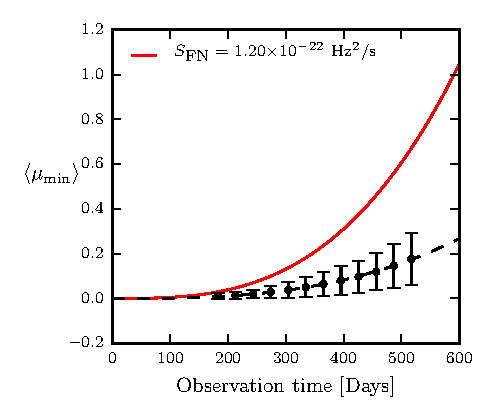
\includegraphics[]{Crab_mismatch_Tobs_with_prediction}
\caption{This figure, updated from Figure~\ref{fig: mismatch Tobs}, shows the
dependence of the minimum mismatch on the observation time for the Crab, along
with the prediction of Eqn.~\eqref{eqn: mu prediction} for the our estimate of
the frequency noise strength parameter calculated in Eqn.~\eqref{eqn: SFN mine}.}
\label{fig: mismatch Tobs update}
\end{figure}
The prediction using the strength parameter calculated from the Crab ephemeris,
as given in Eqn.~\eqref{eqn: SFN mine}, overestimates the dependence of the
mismatch calculated exactly from the data. We feel this is most likely due to timing
noise in the Crab being unlike a random walk. Nevertheless, we have
demonstrated the essential elements of making such predictions which may be useful
in the future, if there is a clear case where the timing noise is well
modelled by a random walk.


%\section{Predicting the mismatch for other pulsars}
%\label{sec: other pulsars}
%\citet{Jones2004} considered the problem of timing noise in pulsars by
%calculating a decoherence time. They then used a fitting formulae from
%\citet{Dewey1989} to predict the strength of timing noise and estimate this
%decoherence time. The fitting formulae is given by defining the activiy
%parameter as the logarithm of the ratio root-mean-square phase residual
%to that of the Crab:
%\begin{align}
%A = \log\left(\frac{\sigma^{2}_{\phi}}{\sigma_{\phi\; \textrm{Crab}}^{2}}\right),
%\end{align}
%then, the fitting formulae is
%\begin{align}
%A = -1.4\log P + 0.8 \log \frac{\dot{P}}{10^{-15}} - 3.31
%\end{align}
%where $P$ is the pulsar's spin period in seconds and $\dot{P}$ is the
%dimensionless period derivative.
%
%From Eqn.~\eqref{eqn: S calc} we can convert this into a prediction for the
%strength of frequency noise
%\begin{align}
%S_{\textrm{FN}} = 10^{2A} S_{\textrm{FN}}^{\textrm{Crab}}
%\label{eqn: SFN prediction}
%\end{align}
%Then, using Eqn.~\eqref{eqn: mu prediction} we can predict the level of mismatch
%for a gravitational wave search for a pulsar.
%
%Many gravitational wave search may be effected by timing-noise, but blind
%searches are particuarly at risk due to the lack of EM information regarding
%the timing properties of the star. This includes all-sky searches along with
%directed searches where a small patch of sky is searches where it is thought
%there may be a neutron star. In Table~\ref{tab: searches} we listed the the
%parameter spaces, coherence times and observation times for several recent
%blind searches. With the exception of the search Cas A, all of these use an
%initial semi-coherent stage. We have not calculated the semi-coherent mismatch
%due to a random walk model of timing noise. However, candidates identified in this
%semi-coherent stage would be followed by a fully-coherent search. To estimate
%how timing noise in the signal may effect this fully-coherent stage, in
%Table~\ref{tab: past search RW} we list the \emph{maximum} predicted metric-mismatch
%for the observation time and search parameters of each search.
%\begin{table}[htb]
%\begin{tabular}{l|l|l|l}
%&\multicolumn{3}{|c|}{\textbf{normal population}} &\multicolumn{3}{|c|}{\textbf{Vela-like population}}\\ \hline
&$\langle N\rangle$&$\langle \tilde{\mu}\rangle$&$\langle \hat{\mu}\rangle$&$\langle N\rangle$&$\langle \tilde{\mu}\rangle$&$\langle \hat{\mu}\rangle$ \\ \hline
S5 E@H all-sky & $2.7$ & ${1.2}\times 10^{4}$ & $0.3$ & $1.2$ & ${9.0}\times 10^{4}$ & $2.7$ \\
S5 E@H galactic center & $6.2$ & ${2.6}\times 10^{5}$ & $7.2$ & $2.6$ & ${5.0}\times 10^{4}$ & $1.5$ \\
%S6 all-sky bucket & $1.1$ & $420.0$ & $0.47$ & $0.48$ & ${1.0}\times 10^{4}$ & $14.0$ \\
S5 all-sky & $0.98$ & $260.0$ & ${9.8}\times 10^{-6}$ & $0.42$ & ${2.0}\times 10^{4}$ & ${9.2}\times 10^{-4}$ \\
VSR low-frequency all-sky & $1.5$ & ${1.2}\times 10^{3}$ & ${3.8}\times 10^{-3}$ & $0.65$ & ${5.9}\times 10^{3}$ & ${2.2}\times 10^{-2}$ \\
S5 supernova remnant (Cas A) & $0.16$ & $3.0$ & $-$ & ${6.8}\times 10^{-2}$ & $12.0$ & $-$ \\
%O1 E@H all-sky & $0.82$ & $140.0$ & $3.7$ & $0.35$ & ${5.3}\times 10^{3}$ & $170.0$ 

%\end{tabular}
%\caption{Predicted worst-case metric-mismatch due to timing noise for the blind
%searches listed in Table~\ref{tab: searches}. These values are calculated by
%taking the maximum absolute frequency and spin-down rate searched for,
%using Eqn.~\eqref{eqn: SFN prediction} to predict the estimated strength of
%timing noise, then calculating the corresponding mismatch from Eqn.~\eqref{eqn:
%mu prediction}.}
%\label{tab: past search RW}
%\end{table}
%From this table, we see that for some searches, the predicted metric-mismatch can be
%greater than one. This indicates that the true mismatch in such a search would be
%large and therefore the signal would be lost. However, we emphasise that these
%are worst-case predictions taken at the corner of parameter space where the
%mismatch is predicted to be the largest. Moreover, it is unclear if the
%fitting formulae of \citet{Dewey1989} is appropriate in these instances. In the
%future, we would like to investigate this issue in more detail and understand
%how these estimates vary the whole search-parameter space.


\section{Conclusion}

In this Chapter, we have calculated the expectation of the fully-coherent
mismatch when searching for a GW signal which undergoes a random walk in one of
the phase, frequency, or spin-down rate. We did this first for a system in
which the difference between the signal and template was initially zero and
then grew as a random walk. Since this is not a minimised result, we then
demonstrated how to minimised the mismatch with respect to the template
parameters $f_\textrm{t}$ and $\dot{f}_\textrm{t}$. The formulae derived in
this section have been verified against Monte-Carlo type simulations of the exact
mismatch.

In Section~\ref{sec: understanding the random walk model}, we related the
random walk model to a more physical compound Poisson random walk. Using this
description, we formulated the two key results of this chapter:
Eqn.~\eqref{eqn: mu prediction phase} and Eqn.~\eqref{eqn: mu prediction}.
These are the expectation of the minimum metric-mismatch due to random walk in
the phase and frequency respectively as a function of the strength of phase and
frequency noise.

Following this, we developed our understanding of random walk models in the
context of the data from the Crab ephemeris. We showed that the frequency noise
strength can be measured from this data and has a value consistent with other
results in the literature. We then demonstrated the use of this derived
prediction of the strength of frequency noise and Eqn.~\eqref{eqn: mu
prediction} to predict the results found in Chapter~\ref{sec: timing noise in
cgw} for the dependence of the mismatch on the observation time. The prediction
is not perfect, but does provide a rough order of magnitude figure of the
expected mismatch.

%Finally, we gave preliminary estimates for the mismatch due to timing noise
%in some typical blind gravitational wave searches. This was done by converting
%the signal parameters into the rotation timing parameters, using the \citet{Dewey1989}
%fitting formulae to estimate the strength of timing noise, and then using
%Eqn.~\eqref{eqn: mu prediction} to predict the levels of mismatch. We
%considered worst-case scenarios and found results which indicates there may be
%an issue for some all-sky searches.

\begin{subappendices}

\section{Summation identities}
\label{sec: summation identities}
In this appendix, we derive two useful summation identities used in
Sec.~\ref{sec: random walk models part I}. First, we have
\begin{align}
\s{b=1}{c}\s{a=1}{b} X_{a} & = \left( X_{1}\right)
 + \left( X_{1} + X_{2} \right) + \ldots  +\left( X_{1} + X_{2}
 + \ldots + X_{c-1} + X_{c}\right)\\
& = c X_{1} + (c-1)X_{2} + \ldots + 2 X_{c-1} + X_{c} \\
& = \s{b=1}{c}(c+1-b)X_{b},
\label{eqn: SI 1}
\end{align}
which is used in deriving Eqn.~\eqref{eqn: delta f n}. Second, we have
\begin{align}
\s{j=1}{i-1}\s{k=1}{j-1}(j-k)X_{k} = & [0] + \left[ X_{1}\right]
+ \left[2X_{1} + X_{2} \right] + \left[3X_{1} + 2X_{2} +X_{3}\right]
+ \ldots  \nonumber \\
& + \left[\left(i-2\right)X_{1} + \left(i-3\right)X_{2}
+ \left(i-4\right)X_{3} + \ldots \right. \nonumber \\
& \left. \hspace{5mm}+ 3X_{i-4} + 2X_{i-3} + X_{i-2}\right]  \\
= & \left(1 + 2 + 3 + \ldots +  (i-4) + (i-3) + (i-2)\right)X_{1} \nonumber  \\
& + \left(1 + 2 + 3 + \ldots +(i-4) + (i-3) \right)X_{2}  \nonumber \\
& + \left(1 + 2 + 3 + \ldots + (i-4) \right)X_{3} + \ldots  \nonumber \\
& + (1 + 2 + 3)X_{i-4} + (1+2)X_{i-3} + X_{i-2}  \\
= & \s{k=1}{i-2}k X_{1} + \s{k=1}{i-3}k X_{2}  + \ldots + \s{k=1}{2}k X_{i-3}
+ \s{k=1}{1}kX_{i-2}  \\
= & \s{j=1}{i-2}\left(\s{k=1}{i-1-j}k\right)X_{j} =
\frac{1}{2}\s{j=1}{i-2}(i-j)(i-j-1)X_{j},
\label{eqn: SI 2}
\end{align}
which is used in deriving Eqn.~\eqref{eqn: delta phi n}.


\section{Least-squares minimisation of a random walk}
\label{sec: least squares minimisation of a random walk}
In this appendix, we will describe the process of fitting and
removing a polynomial from $N$ data points $(x_i, y_i)$ which undergoes a
random walk. The polynomial will be fitted using a least squares minimisation.
The $x_i$ are the independent points at which $y_i$ (which undergoes a random
walk) is measured. We begin by defining the least-squares fitting method then
go on to calculate the residual for several different degrees of polynomial.
This introduces the method in a generic setting which is then applied in
Section~\ref{sec: random walk models part II} to calculate the mismatch for a
GW signal which undergoes a random walk, but in which the search minimises the
mismatch over the search frequency and frequency derivative.

\subsection{Least squares fitting of a polynomial}
Given $N$ data points $x_{i}$, $y_{i}$, we define the residual from a least-squares
polynomial fit of order $k$, as
\begin{equation}
    r_i^{(k)} = y_{i} - y^{\textrm{(k)}}_{i},
\end{equation}
where
\begin{equation}
y^{\textrm{(k)}}_{i} = a_{0} + a_{1}x_{i} + a_{2}x_{i}^{2} + \dots
                                                           + a_{k} x_{i}^{k},
\end{equation}
is a polynomial of degree $k$.

Then the residual which we want to minimise is
\begin{equation}
R^{2} = \s{i=1}{N}\left(r_i^{(k)}\right)^{2}
      = \s{i=1}{N}\left(y_{i} - \left(a_{0} + a_{1}x_{i} + a_{2}x_{i}^{2} +
        \dots + a_{k} x_{i}^{k}\right)\right)^{2}.
\end{equation}
Partial differentiation with respect to the parameters $a_{i}$, yields $k$
simultaneous equations. Writing these as a matrix and then solving
for the best fit, $\hat{y}^(k)_i$, it can be shown (see for example
\citeauthor{WolframLeastSquares}) that
\begin{align}
\hat{y}^{\textrm{(k)}}_{i} & = X \left(X^{T}X\right)^{-1} X^{T} y_{i} & \textrm{where} & &
X & = \left[\begin{array}{ccccc}
1 & x_{1} & x_{1}^{2} & \dots & x_{1}^{k} \\
1 & x_{2} & x_{2}^{2} & \dots & x_{2}^{k} \\
\vdots & \vdots & \vdots & \vdots & \vdots \\
1 & x_{n} & x_{n}^{2} & \dots & x_{n}^{k} \\
\end{array}\right]
\end{align}
Here $X$ is an example of a \emph{Vandermonde} matrix in which the terms follow
a geometric progression. It is useful to note that
\begin{equation}
XX^{T} = \left[\begin{array}{cccc}
N & \s{i=1}{N}x_{i} & \cdots &  \s{i=1}{N}x_{i}^{k} \\
\s{i=1}{N}x_{i} & \s{i=1}{N}x_{i}^{2} & \cdots &  \s{i=1}{N}x_{i}^{k+1} \\
\vdots & \vdots & \ddots & \vdots \\
\s{i=1}{N}x_{i}^{k} & \s{i=1}{N}x_{i}^{k+1} & \cdots &  \s{i=1}{N}x_{i}^{2k}
\end{array}\right].
\end{equation}

Provided that the $x_{i}$ are suitably defined, then an analytic fit can be
found for any $k$, the difficulty lies in inverting the matrix.

\subsection{Least squares fitting a polynomial to a random walk} We now take
the $x_i, y_i$ to be a Gaussian random walk beginning at the origin. To define
this, let $\tn y_{i} \sim N(0, \sigma^{2})$ be independent and identically
distributed random variables for which their sum generates the random walk:
\begin{equation}
y_{i} = \sum_{j=1}^{i}\tn y_{i}.
\label{eqn: ToyModel RW definition}
\end{equation}
We also set each random walk event to occur according to $x_{i} = i \Delta x$.
Then the residual after fitting and removing a $k^{th}$ order polynomial to the
random walk $y_i$, is
\begin{equation}
r_i^{(k)} = y_{i} - \hat{y}_{i}^{(k)} = y_{i} - X \left(X^{T}X\right)^{-1} X^{T} y_{i}.
\label{eqn: fitted residual}
\end{equation}
This suggests the residual will be similar to the random walk, but modified by
the least squares fitting.  To illustrate this, in Figure~\ref{fig: ToyModelRW}
we plot a simulated random walk along with several fits.
\begin{figure}[htb]
\centering
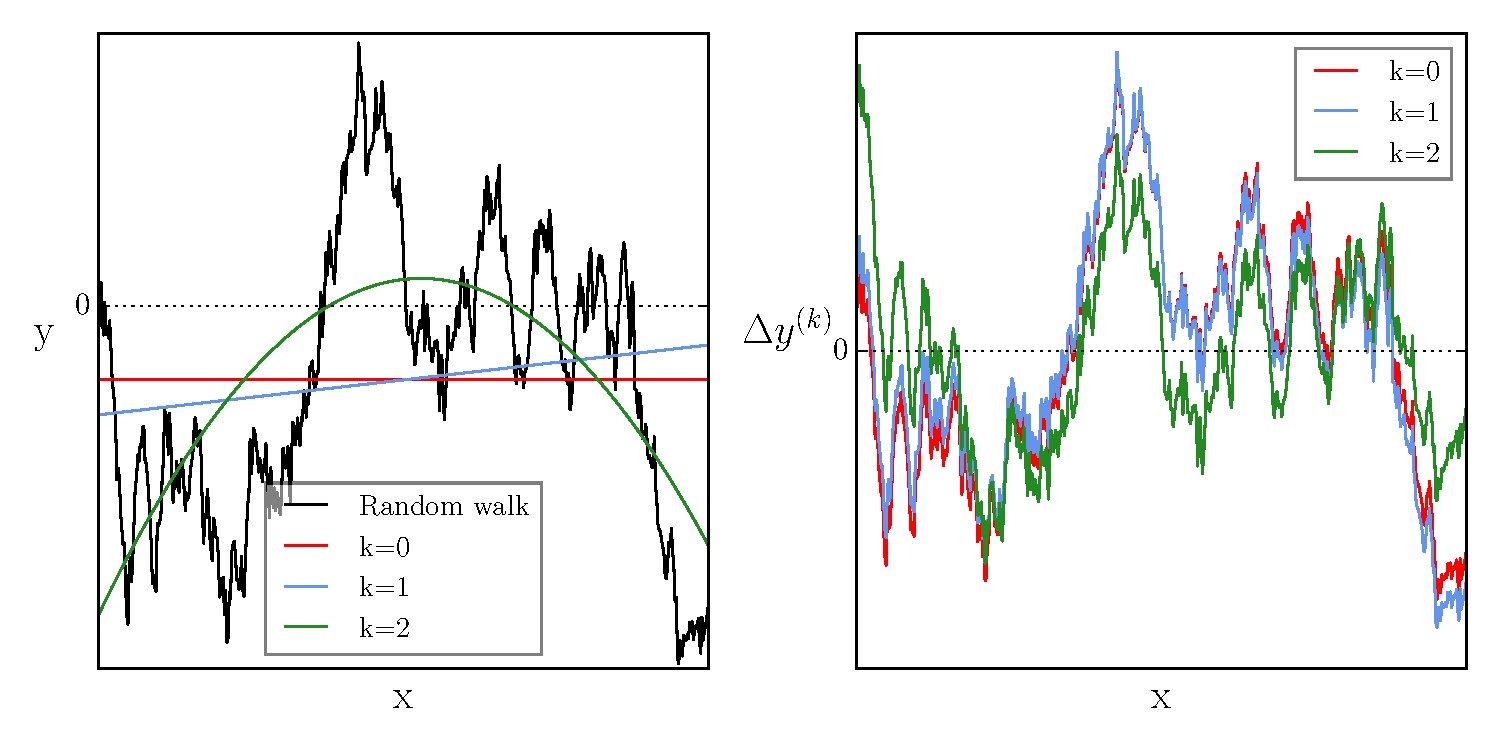
\includegraphics[width=.9\textwidth]{ToyModelRW}
\caption{Example of a random walk on the left along with three polynomial fits
of varying order. On the right is the corresponding residual after subtracting
these fits. A dotted line marks the origin in both plots.}
\label{fig: ToyModelRW}
\end{figure}

\subsection{Zeroth order fitting}

We begin with the case of $k=0$ in which $X^{T} = [1, 1, \dots 1]$ such
that
\begin{equation}
X \left(X^{T}X\right)^{-1} X^{T} = \frac{1}{N} J_{N}
\end{equation}
where $J_{N}$ is the $N\times N$ matrix of ones.  Inserting this into
Eqn.~\eqref{eqn: fitted residual}, the residual from a zeroth order fit is
given by
\begin{equation}
r_i^{(0)}= y_{i} - \frac{1}{N} \s{j=1}{N}y_{j}.
\end{equation}
The zeroth order residual can be interpreted as the removing the
average value $\langle y_i \rangle$ from the random walk: this was illustrated
in Figure~\ref{fig: ToyModelRW}.

%For example the
%expectation after $i$ steps of the original random walk can be shown to be
%zero, therefore the expectation for the zeroth order residual after $i$ steps
%will also be zero.

%This can intuitively be understood from the fact that we started out RW at the origin,
%a zeroth order fit shifts the origin but a random walk should

We can now take expectations to understand the behaviour of the residual when
compared to the original definition of the random
walk in Eqn.~\ref{eqn: ToyModel RW definition}. For example, consider
the mean square translation distance from the origin of a random walk after $i$
steps. For a normal random walk, this has the well known result
\begin{equation}
E[y_{i}^{2}] = i \sigma^{2}.
\label{eqn: RW classic}
\end{equation}
We can calculate the corresponding quantity of the $k=0$ residual by first
noting that
\begin{align}
E\left[y_{i}y_{j}\right] & = E\left[\s{k=1}{i}\tn y_{k} \s{l=1}{j}\tn y_{l} \right] \\
& = \s{k=1}{i}\s{l=1}{j}E\left[\tn y_{k} \tn y_{l}\right] \\
& = \s{k=1}{i}\s{l=1}{j} \delta_{kl} \sigma^{2} \\
& = \sigma^{2}\min(i, j),
\label{eqn: E yiyi}
\end{align}
where $\delta_{kl}$ is the Kronecker delta. Then we have
\begin{align}
\left(r^{(0)}_{i}\right)^{2} & = y_{i}^{2} - \frac{2}{N}\s{k=1}{N}y_{i}y_{k} + N^{-2}\s{k=1}{N}\s{l=1}{N}y_{k}y_{l} \\
& =  y_{i}^{2} - 2 N^{-1} \left(\s{k=1}{i}y_{i}y_{k} + \s{k=i+1}{N}y_{i}y_{k} \right)+ N^{-2}\s{k=1}{N}\left(\s{l=1}{k}y_{k}y_{l} + \s{l=k+1}{N}y_{k}y_{l} \right).
\end{align}
Taking the expectation we have
\begin{align}
E\left[\left(r^{(0)}_{i}\right)^{2} \right] & = \sigma^{2}\left(i - \frac{2}{N}\left(\s{k=1}{i}k + \s{k=i+1}{N}i \right)+ \frac{1}{N^{2}}\s{k=1}{N}\left(\s{l=1}{k}l+ \s{l=k+1}{N}k \right) \right) \\
& = \sigma^{2}\left(\frac{N}{3} - i + \frac{1}{2} + \frac{i^{2}}{N} - \frac{i}{N} + \frac{1}{6 N}\right).
\end{align}
This result can be compared with Eqn.~\eqref{eqn: RW classic}, the expectation
of the squared value for a random walk.  In contrast, the expectation after $i$
steps for the residual random walk depends on the length of data $N$ that was
fitted. It can be shown the expectation has a minimum at $i=N/2$.

To further understand the difference between the random walk and
the residual random walk, let us consider the sum of squares after $N$ steps for
the random walk
\begin{equation}
E\left[\s{i=1}{N} y_{i}^{2}\right] = \s{i=1}{N} i \sigma^{2} =
                               \frac{1}{2}\left(N^{2} + N\right)\sigma^{2}.
\label{eqn: sum of squares}
\end{equation}
On the other hand, the sum of squares for the residual random walk is given by
\begin{equation}
E\left[\s{i=1}{N} \left(r^{(0)}_{i}\right)^{2}\right] =
\frac{1}{6}\left(N^{2} -1\right)\sigma^{2}.
\label{eqn: sum of squares k0}
\end{equation}
Comparing equations \eqref{eqn: sum of squares} and \eqref{eqn: sum of squares
k0} we note that, for the leading order term, the coefficient is reduced, but
the power remains the same.

%We verify this behaviour with a simple script that produces a random walk of
%length $N$ then fits and subtracts a $0^{th}$ order polynimial; we then
%calculate the sum of the square residual. In Figure~\ref{fig:
%sum_of_squares_res_oth_order} we repeat this operation multiple times then plot
%the average of the sum of squares for the residual while varying $N$, the
%prediction of Eqn.~\eqref{eqn: sum of squares k0} is also plotted showing
%agreement.
%
%\begin{figure}[ht]
%\centering
%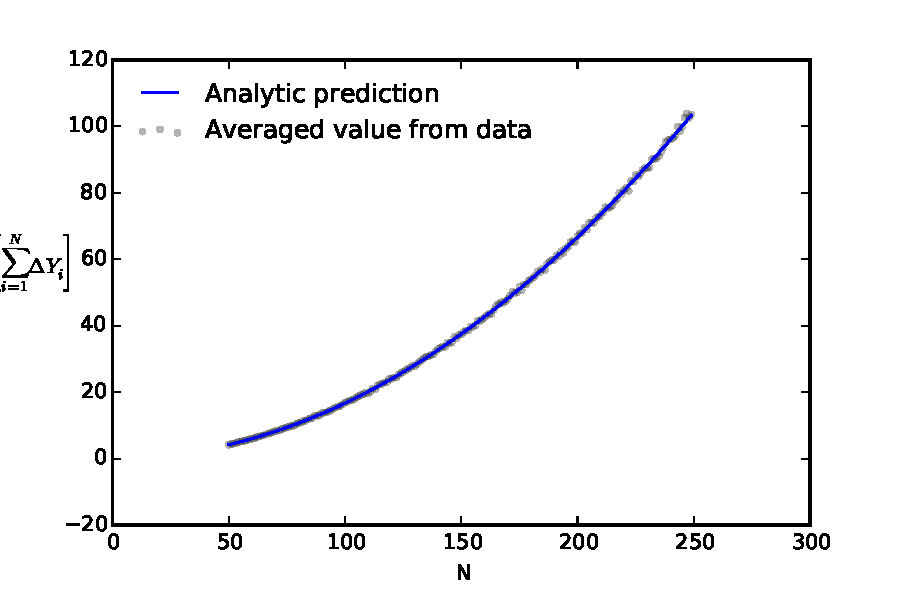
\includegraphics[width=.6\textwidth]{sum_of_squares_res_oth_order}
%\caption{Comparing Eqn.~\eqref{eqn: sum of squares k0} with the averaged sum of squares for a simulated random walk }
%\label{fig: sum_of_squares_res_oth_order}
%\end{figure}

\subsection{First order fitting}
We now consider a first order fitting for which
\begin{align}
\hat{y}^{(1)}_{i} & = X\left(X^{T}X\right)^{-1} X^{T} y_{i} & \textrm{with} &&
X & = \left[\begin{array}{cc}
1 & \Delta x \\
1 & 2 \Delta x  \\
\vdots & \vdots  \\
1 & N \Delta x  \\
\end{array}\right].
\end{align}
Inserting the definitions of $x_{i}$ we can write
\begin{equation}
\left(X^{T}X\right)^{-1} = \frac{1}{N(N-1)}\left[
\begin{array}{cc}
4N+2 & -\frac{6}{\Delta x} \\
 -\frac{6}{\Delta x} & \frac{12}{\Delta x^{2} (N+1)}
\end{array}•
\right] = \Cone.
\end{equation}
For convenience we have defined a symmetric matrix $\Cone$. We then proceed to
define another matrix
\begin{align}
    \mathcal{C}_{ij}^{(1)} & := X\Cone X^{T} \\  & =
\left[\begin{array}{cc}
1 & \Delta x \\
1 & 2\Delta x  \\
\vdots & \vdots  \\
1 & N \Delta x \\
\end{array}\right]
\left[\begin{array}{cc} \Cone_{11} & \Cone_{12} \\ \Cone_{21} & \Cone_{22} \end{array}\right]
\left[\begin{array}{cccc}
1 & 1 & \dots & 1 \\
\Delta x & 2\Delta x & \dots  & N \Delta x
\end{array}\right] \\
& =
\Cone_{11} J_{N} +
\Cone_{12} \Delta x \left[ \begin{array}{cccc}
2 & 3 & \dots & N+1 \\ 3 & 4 & \dots & \vdots \\ \vdots & & & \\  N+1& \dots & \dots & 2N
\end{array}\right] +
\Cone_{22} \Delta x^{2} \left[ \begin{array}{cccc}
1 & 2 & \dots & N \\ 2 & 4 & \dots & \vdots \\ \vdots & & & \\  N& \dots & \dots & N^{2}
\end{array}\right]
\end{align}
We can write $r^{(1)}_{i}$ as a summation by inferring the dependence of the
$i^{th}$ row of each matrix on the $j^{th}$ column
\begin{align}
r^{(1)}_{i} & = y_{i} - \s{j=1}{N}\mathcal{C}_{ij}^{(1)} y_{j}
& \textrm{ where} &&
\mathcal{C}_{ij}^{(1)} & = \Cone_{11} + \Cone_{12}\Delta x (i+j) + \Cone_{22}\Delta x^{2} ij
\end{align}

We have now defined the first order residual. To understand that fitting an
removing a first order polynomial has, we compute the expectation of the
square for the $i^{th}$ term
\begin{align}
\begin{split}
E\left[\left(r^{(1)}_{i}\right)^{2}\right]  =
\frac{1}{15 N \left(N^{2} - 1\right)} &
\left(2 N^{4} - 18 N^{3} i + 9 N^{3} + 78 N^{2} i^{2} - 78 N^{2} i \right.\\
      &\hspace{3mm} + 14 N^{2} - 120 N i^{3} + 180 N i^{2} - 78 N i \\
      &\hspace{3mm} \left. + 9 N + 60 i^{4} - 120 i^{3} + 78 i^{2} - 18 i + 2\right),
\end{split}
\end{align}
which can be compared with the classic result for a random walk given in
Eqn.~\eqref{eqn: RW classic}. Alternatively, comparing with Eqn.~\eqref{eqn:
sum of squares}, the expected sum of squares for the residual random walk is
\begin{equation}
E\left[\s{i=1}{N} \left(r^{(1)}_{i}\right)^{2}\right]
= \frac{1}{15}\left(N^{2} -4\right)\sigma^{2},
\label{eqn: sum of squares k1}
\end{equation}
as in the zeroth order fit, the power of the leading order term remains the
same, but the coefficient decreases.

\subsection{Second order fitting}
For the residual left after removing a quadratic, the  argument proceeds in much
the same way with
\begin{align}
r^{(2)}_{i} & = y_{i} - \s{j=1}{N}\mathcal{C}_{ij}^{(2)} y_{j},
\end{align}
where
\begin{align}
\mathcal{C}_{ij}^{(2)}  = &\Ctwo_{11} + \Ctwo_{22}\Delta x^{2}ij +
\Ctwo_{33}\Delta x^{4}i^{2}j^{2} \nonumber + \Ctwo_{12}\Delta x(i+j) \nonumber \\
& + \Ctwo_{13}\Delta x (i^{2} + j^2) + \Ctwo_{23}\Delta x^{3}(ij^{2} + i^{2}j),
\label{eqn: MC_2}
\end{align}
and
\begin{equation}
C^{(2)} = \frac{1}{N(N-1)(N-2)}
\left[\begin{matrix}9 N^{2} + 9 N + 6 & - \frac{1}{\Delta{x}} \left(36 N + 18\right) & \frac{30}{\Delta{x}^{2}}\\- \frac{1}{\Delta{x}} \left(36 N + 18\right) & \frac{12 \left(2 N + 1\right) \left(8 N + 11\right)}{\Delta{x}^{2} \left(N + 1\right) \left(N + 2\right)} & - \frac{180}{\Delta{x}^{3} \left(N + 2\right)}\\\frac{30}{\Delta{x}^{2}} & - \frac{180}{\Delta{x}^{3} \left(N + 2\right)} & \frac{180}{\Delta{x}^{4} \left(N + 1\right) \left(N + 2\right)}\end{matrix}\right].
\label{eqn: C_2}
\end{equation}

The expression for the expected square value is too long to write out in full,
but the expected sum of squares for the residual random walk is
\begin{equation}
E\left[\s{i=1}{N} \left(r^{(2)}_{i}\right)^{2}\right] =
 \frac{1}{70}\left(3N^{2} -27\right)\sigma^{2},
\label{eqn: sum of squares k2}
\end{equation}
for which as in the case of the zeroth order and first order residuals, the
power of the leading order term remains unchanged, but the coefficient
decreases.

\subsection{Conclusions}
\label{sec: appendix conclusions}
We now have a method to calculate statistical quantities from the residual
left over after subtracting a $k^{th}$ order polynomial from a random walk.
Considering the sum of squares for a random walk and the residuals in equations
\eqref{eqn: sum of squares}, \eqref{eqn: sum of squares k0},
\eqref{eqn: sum of squares k1}, and \eqref{eqn: sum of squares k2} we find that
the leading order term retains the same
power of $N$ with increasing $k$ but the coefficient of this power gets
smaller. This reflects the improved fitting with the polynomial degrees. We
also note that with each increase in the order of fit we get a limit
on $N$ for which the sum of squares is positive. For zeroth order fitting this
is $N>1$, for first order $N>2$ and for second order $N>3$. This is because in
order to perform a least squares fit, we need at least $k+1$ points to fit.

\end{subappendices}


\biblio

\end{document}
